\chapter{Úvod}
Schopnost dorozumět se s~ostatními lidmi na planetě je nesmírně důležitá, české přísloví dokonce praví \uv{Kolik řečí znáš, tolikrát jsi člověkem}. Proto učenci od pradávných let vytvářeli slovníky a vědci od vzniku výpočetní techniky zkoumají jak vytvořit kvalitní překladový systém.

Ideálem je překlad tak, jak ho známe ze science fiction materiálů. Dvě osoby, mluvící jiným jazykem, si navzájem rozumí v~reálném čase. S~intenzivním rozvojem strojového učení a umělé inteligence, který nastal v~posledních letech, se k~tomuto ideálu blížíme mílovými kroky. Automatické rozpoznání mluvené řeči je již dostupné v~běžných spotřebitelských zařízeních a automatický překlad se taky značně vylepšuje.

Obsahem této práce je popis a realizace takového automatického překladového systému. Systém by měl být schopný naučit se za pomocí velkého množství zarovnaných vět v~různých jazycích překládat věty mezi těmito jazyky. K~tomu je použita architektura rekurentních neuronových sítí enkodér-dekodér, která vykazuje v~posledních letech dobré výsledky.

V~následující kapitole \ref{chapter:theory} je popis překladového systému a jsou zde rozebrány důležité pojmy a teorie ze kterých je je systém vystavěn. Větší část této kapitoly vznikla v~rámci semestrálního projektu. Kapitola \ref{chapter:implementation} popisuje implementovaný systém a kapitola \ref{chapter:results} podává výsledky experimentů s~vytvořeným systémem a porovnává je s~výsledky podanými nástrojem pro statistický překlad Moses.

Vytvořený balíček je publikovaný na serveru github na adrese \url{github.com/jojkos/neural-machine-translation}.


\chapter{Strojový překlad}\label{chapter:theory}
Účelem této kapitoly je blíže vysvětlit a rozebrat jednotlivé pojmy a komponenty potřebné pro vytvoření překladového systému.

\section{Popis cílového systému} \label{chapter:draft}
Cílem této práce práce je vytvořit systém pro strojový překlad textu pomocí umělých neuronových sítí. Pro snadnou představu, je to podobné tomu co dělá Google Translator\footnote{\url{translate.google.cz}} -- blíže popsáno v~článku \cite{googleBridgingGap}. Vezme se věta v~původním jazyce a vytvoří se z~ní co nejvěrnější překlad v~jazyce cílovém a to za pomocí natrénované rekurentní neuronové sítě. V~této sekci je vysvětleno, jak by takový systém mohl vypadat a jaké komponenty potřebuje k~tomu, aby fungoval.

\begin{description}
  \item[Dataset:] Aby bylo možné natrénovat neuronovou síť pro překlad, je nejprve zapotřebí mít dataset. Dataset obsahuje texty ve dvou jazycích, mezi kterými se má překládat. Tyto texty musí být zarovnané tak, aby si jednotlivé věty v~těchto jazycích navzájem odpovídaly. Obecně platí, že čím větší množství použitých dat a čím větší model, tím lepší bude výsledek (článek \cite{googleLimits}).

  \item[Tokenizer:] Dataset a jeho jednotlivé věty je nejprve potřeba před začátkem trénování sítě připravit. Tokenizer rozdělí věty na jednotlivé tokeny a zahodí zvolené nepodstatné vlastnosti, například velká písmena na počátku vět nebo interpunkce. To usnadňuje práci s~datasety a také snižuje velikost slovníků.

  \item[Slovník:] Slovník se vytvoří jako seznam $n$ nejčastějších slov v~datasetu, ve vstupním a cílovém jazyce. Čím je slovník menší, tím jsou menší požadavky na vypočetní výkon. Na druhou stranu je pak potřeba vyřešit při trénování a překladu problém se slovy nevyskytujícími se ve slovníku (popsáno v~sekci \ref{subsection:oov}).

  \item[Word Embeddings:] Obecně je možné vytvářet jazykové modely, které generují text po písmenech, částech slov nebo po slovech \cite{mikolovSubwords}. Word embeddings je další forma předzpracování. Každý token ze vstupního slovníku se převede do vektoru reálných čísel, ve kterém jsou zakódovány některé syntaktické a sémantické vlastnosti daného tokenu, což umožní neuronové síti se učit lépe, než kdyby se použilo například jenom číslo označující pozici tokenu ve slovníku. Více v~sekci \ref{subsection:neuralembeddings}.

  \item[Model:] V~současné době nejúspěšnější architekturou používanou pro překlad je enkodér-dekodér umožňující překlad po celých větách (sequence to sequence, dále seq2seq \cite{seq2seq}). To je rozdíl oproti starším statistickým metodám překladu, kde se překládalo po slovech či frázích.

      Nejprve enkodér vezme word embedding na vstupu a pomocí rekurentní neuronové sítě (sekce \ref{section:rnn}) převede větu na vstupu do velkého vektoru reprezentujícího její význam (tzv. myšlenkový vektor -- intuice je taková, že když člověk překládá větu, také nejprve pochopí její význam a až poté ji začne překládat). Dekodér -- taky rekurentní neuronová síť -- následně z~tohoto vektoru slovo po slovu vygeneruje výslednou přeloženou větu. Dekodér tedy funguje jako jazykový model (sekce \ref{section:langmodel}), který je inicializovaný na jednu konkrétní větu.
\end{description}


\begin{figure}[H]
    \begin{center}
            \tmpframe{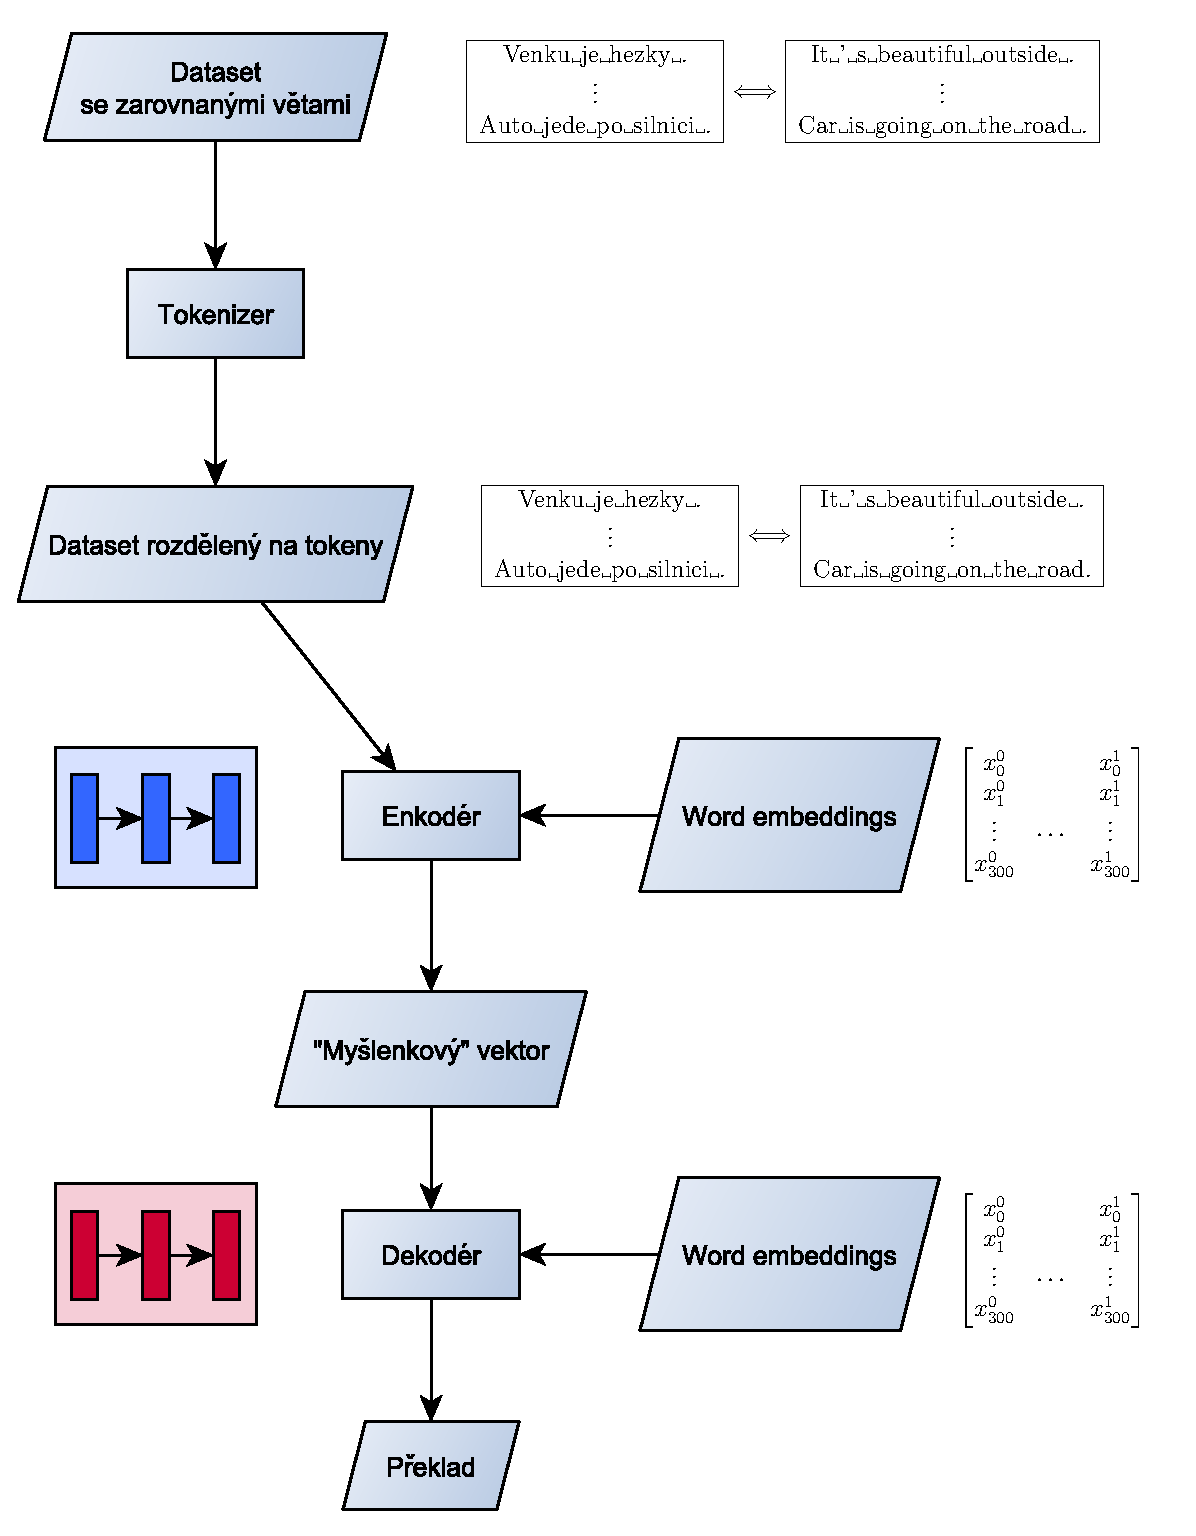
\includegraphics[width=0.75\linewidth]{img/graphs/draftEnhanced.pdf}}
    \end{center}
	\caption{Schéma návrhu systému pro překlad. Dataset se předzpracuje pomocí tokenizeru. Do enkodéru vstupují tokeny převedené na embeddings. Enkodér větu zakóduje do velkého "myšlenkového" vektoru, ze kterého dekodér generuje překlad.}
	\label{img:draft}
\end{figure}



\section{Jazykové modely}\label{section:langmodel}
Zatímco u~programovacích jazyků existuje formální definice přesně popisující jejich syntax a význam, u~přirozených jazyků to tak není. Přirozený jazyk vznikl náhodným způsobem v~průběhu staletí a tisíciletí narozdíl od formálně definovaných jazyků, které byly precizně navrženy. Přestože běžný jazyk se řídí nějakými pravidly, existuje značné množství výjimek a odchylek. I~napříč tomu si však lidé navzájem rozumí. Problém však je tato neurčitá pravidla převést do formálních pravidel tak, aby jim rozuměl počítač. Řešením pro tento problém mohou být jazykové modely, které nevznikají nadefinováním formálních pravidel, ale natrénováním modelu z~příkladů. Sekce vychází z~práce \cite{nmtThesis} a článku \cite{nmtTutorial}.
\\\\
Jazykový model udává pro každou větu $w$ jaká je její pravděpodobnost. Respektive pro sekvenci slov $w = w_1, w_2..., w_m$ získá pravděpodobnost podle rovnice \ref{figure:probdistr}.

\begin{align}\label{figure:probdistr}
  p(w) = \prod_{i=1}^{m} p(w_i|w_{<i})
\end{align}

Pro každé slovo $w_i$ ze sekvence $w$ určí, jaká je jeho podmíněná pravděpodobnost v~případě, že se před ním nachází slova $w_{<i}$.

\subsection{N-gram modely}\label{subsection:ngram}
Ve výsledku je pro překladový systém potřeba získat model, který pro zdrojovou větu $F$ vrátí přeloženou větu $E$, tak že $P(E|F)$. N-gram model je však jazykový model, který udává jen pravděpodobnost věty P(E) (pro nějaký daný kontext nad kterým se model natrénoval).

Takovýto model umožní zhodnotit přirozenost věty a generovat text podobný tomu, na kterém byl model nacvičen.

\begin{description}
  \item[Zhodnocení přirozenosti:] Pomocí jazykového modelu je možné pro větu $w$ zhodnotit, jak moc je přirozená neboli jak moc je pravděpodobné, že by takováto věta mohla existovat v~textu, na kterém byl model natrénován.
  \item[Generování textu:] Protože model umožňuje pro každé slovo $w_i$ získat pravděpodobnost následujícího slova $w_{i+1}$, je takto možné generovat náhodný, přirozeně (vůči zdrojovému textu) vypadající text. Přesně tato vlastnost je potřeba pro generování překladů.
\end{description}

$N$-gram modely umožňují určit pravděpodobnost následujícího slova ve větě v~případě, že se před ním nacházelo $n$ nějakých slov (rovnice \ref{figure:ngram}).

\begin{align}\label{figure:ngram}
    P(x_{i}\mid x_{{i-(n-1)}},\dots ,x_{{i-1}})
\end{align}

Se zvětšujícím se $n$ se výrazně zvětšuje náročnost výpočtu. Tímto způsobem tak není snadné zachytit závislosti mezi slovy vzdálenými od sebe více než několik málo míst.

\subsection{Log-lineární modely} \label{subsection:loglinear}
Stejně jako v~případě $n$-gram modelů (sekce \ref{subsection:ngram}), tyto modely počítají pravděpodobnost následujícího slova $w_i$ při kontextu $w_{<i}$. $N$-gram model počítá pouze s~výskytem (identitou) slova. Log-lineární modely pracují s~\textbf{rysy} (z~anglického features). Rys je něco užitečného ohledně daného slova, co se dá použít pro zapamatování a pro předpověď slova dalšího. Jak už bylo řečeno, u~n-gram modelů to je pouze identita minulého slova. Formálněji je rys funkce $\phi(e^{t-1}_{t-n+1})$, která dostane na vstupu aktuální kontext a jako výsledek vrátí reálnou hodnotu -- vektor rysů $x \in \mathbb{R}^N$ popisující kontext při použití $N$ různých rysů.

Stejně jako u~$n$-gram modelů nastává problém, když je potřeba zaznamenat vzdálenější závislosti. Například u~věty \uv{farmář jí steak} je potřeba zaznamenat pro předpovězení slova \uv{steak} jak jeho předcházející slovo $w_{t_1}=j\acute{\imath}$, tak $w_{t_2}=farm\acute{a}\check{r}$. V~případě, že by se použil pouze rys $w_{t_1}$, mohl by model předpovídat i věty, které nedávají smysl. Jako je například \uv{kráva jí steak}. Při použití většího množství rysů vznikají mnohem větší nároky na paměť a výkon a taky na velikost trénovacího datasetu. Řešením těchto problémů může být použití neuronových sítí (sekce \ref{subsection:neuralembeddings}).


\subsection{Neuronové sítě a word embeddings}\label{subsection:neuralembeddings}
Stejně jako předchozí modely i NLM (neural language model) je trénován tak, aby předpovídal rozdělení pravděpodobností přes slova v~cílovém slovníku na základě aktuálního kontextu (rovnice \ref{figure:probdistr}).

Předchozí modely při použití většího datasetu a tím pádem většího slovníku čelí \uv{prokletí} dimenzionality. Jednotlivá slova jsou běžně reprezentována jako \textbf{one-hot vektor} (obrázek \ref{figure:oneHot}). Pro reprezentaci jednoho slova je tak použit rozsáhlý vektor $x_i \in \mathbb{R}^{V}$, kde $V$ je použitý slovník daného jazyka. Většina hodnot, až na hodnotu označující dané slovo, je nulová (řídký vektor neboli sparse vector).

\begin{figure}[H]
    \begin{center}
        $V$ = $[$farmář, jí, steak, kráva$]$ \quad
        $
        oneHot_{steak}=
        \begin{bmatrix}
            0 \\
            0 \\
            1 \\
            0 \\
        \end{bmatrix}
        $
    \end{center}
	\caption{One-hot vektor pro slovo \uv{steak} ze slovníku $V$. Slovo je znázorněno jedničkou na třetí pozici, což odpovídá jeho pozici ve slovníku. Všechny ostatní pozice vyplňují pouze nuly (řídký vektor). Pro velký slovník to znamená, že každé slovo zabere značné množství paměti.}
	\label{figure:oneHot}
\end{figure}


NLM se s~tímto problémem vypořádává za pomocí takzvaných \textbf{word embeddings}. Word embeddings jsou na rozdíl od one-hot vektoru vektory reálných čísel (husté neboli dense vektory), ukázka v obrázku \ref{figure:wordEmbedding}. Ke každému slovu ze slovníku se přiřadí takovýto vektor. Výhodou je, že může nést, na rozdíl od pouhé pozice slova ve slovníku, další různé užitečné významy. Třeba pro slovo \uv{kráva} by ve vektoru mohly být zakódované významy jako podstatné jméno, velký savec atd. Díky tomu může model lépe generalizovat a slova, která mají sobě blízké vektory, může model brát například jako synonyma.

\begin{figure}[H]
    \begin{center}
        $V$ = $[$farmář, jí, steak, kráva$]$ \quad
        $
        wordEmbedding_{steak}=
        \begin{bmatrix}
            x_0 \\
            x_1 \\
            $\vdots$ \\
            x_{300} \\
        \end{bmatrix}
        $
    \end{center}
	\caption{Word embedding vektor pro slovo \uv{steak} ze slovníku $V$. Slovo je vyjádřeno vektorem o~velikosti 300, který v~sobě může uchovávát některé jeho sémantické vlastnosti.}
	\label{figure:wordEmbedding}
\end{figure}

Nejznámější ukázkou vlastností word embeddings je ukázka \ref{figure:kingQueen} z~článku \cite{kingQueen}.


\begin{figure}[H]
    \begin{center}
        $
          v(kr\acute{a}l) - v(mu\check{z}) + v(\check{z}ena) \approx v(kr\acute{a}lovna)
        $
    \end{center}
	\caption{Ukázka vlastností word embeddings. $\approx$ udává nejbližšího souseda v~prostoru. Je vidět, že vektory v~sobě nesou určitý sémantický význam. Odečtením hodnoty vektoru slova \uv{muž} se získá jakási podstata slova \uv{král} nebo \uv{kralovat}. Přičtením hodnoty slova \uv{žena} k~této dočasné hodnotě se pak získá ženská varianta krále -- královna.}
	\label{figure:kingQueen}
\end{figure}


Existuje několik variant výpočtů word embeddings -- word2vec \cite{word2vec}, glove \cite{glove} a fasttext \cite{fasttext}.


Embbedings jsou vhodné pro \textbf{transfer learning}. To je způsob využití znalostí natrénovaných již třeba dříve pro jiný problém. Word embeddings je možné buďto získat v~průběhu učení modelu nebo použít už předtrénované, připravené pro tento účel. Díky tomu může model získat více znalostí o~jednotlivých slovech a celkový výsledek tak může být výrazně lepší.

\subsection{Zpracování neznámých slov} \label{subsection:oov}
Jazykový model typicky pracuje s~pevně danou velikostí slovníku (počtem slov, co se mohou vyskytovat), což je problém, protože překlad je obecně problém s~otevřenou slovní zásobou. Existuje-li dataset $\varepsilon_{train}$ obsahující texty na kterých se model bude učit a dataset $\varepsilon_{test}$, který bude sloužit k~ověření výkonnosti a generalizace modelu, je více než pravděpodobně, že v~testovacím setu se budou nacházet slova, která se v~trénovacím nenacházela. To znamená, že se v~testovacím datasetu budou vyskytovat \textbf{neznámá slova}. Pro pokrytí co největšího množství slov by tak bylo potřeba učit model s~co největším slovníkem. To by ale bylo neefektivní a tak naopak může být vhodné pro zlepšení výkonu, omezit celkový počet slov, se kterými se bude model pracovat. Tím pádem se však zvýší výskyt neznámých slov. Práce \cite{nmtTutorial} uvádí tři běžné způsoby, jak se vypořádat s~neznámými slovy.

\begin{description}
  \item[Předpokládat, že slovník je konečně velký:] V~některých případech se dá počítat s~tím, že slovník je omezený. Tím pádem se neznámá slova nebo znaky nemohou vyskytovat. Například, kdyby se trénoval model pouze na znacích ASCII, tak při dostatečně velkém vstupním datasetu by bylo rozumné předpokládat, že se v~něm vyskytly všechny znaky a model se je tedy mohl všechny naučit.
  \item[Interpolovat pravděpodobnost pro neznámá slova:] Je možné interpolovat rozdělení pravděpodobnosti i přes neznámá slova. Lze natrénovat jazykový model,který by po písmenech odhadoval neznámá slova nebo lze odhadnout celkový počet slov ve slovníku a pravděpodobnost $P_{unk}$ pak počítat jako $P_{unk}(e_t) = 1/|V_{all}|$.
  \item[Přidáním speciálního slova <unk>:]\label{description:unk}V případě, že se v~trénovacím setu $\varepsilon_{train}$ některá slova vyskytují málo nebo jenom jednou, mohou se nahradit speciálním slovem \emph{<unk>}. S~tímto slovem se pak pracuje stejně jako s~ostatními. Díky tomu se zredukuje počet slov ve slovníku a tedy náročnost výpočtu. Má však přiřazenou svoji pravděpodobnost a může se tak vyskytnout v~předpovědi modelu při generování textu.
\end{description}

Dalším uváděným řešením je místo slov jako nejmenších tokenů, se kterými se pracuje, použití takzvaných \textbf{subword units} neboli jednotek menších než slovo \cite{subwords}.

\begin{description}
  \item[Subword units:]\label{subsection:subwords} Kvůli velkému množství slov a jejich tvarů se obvykle používá velikost slovníků kolem 30 000--50 000 slov. Kvůli tomu je trénink a překlad náročnější a také to nezaručuje kvalitní překlad pro vzácná slova, ani že se nevyskytnou slova neznámá. Značné množství slov je tvořeno několika z několika částí, předložkami a spojenými slovy (například \uv{kladkostroj}). Ukázalo se, že v~případě, že se slova rozdělí na takovéto podčásti, tak se:

      \begin{enumerate}
        \item Zmenší velikost slovníku - kdyby se místo slov pro trénování sítě používala jednotlivá písmena, velikost slovníku by byla samozřejmě nejmenší, ale trénink modelu by byl složitý. Při použití částí slov je možné z~nich skládat větší celky a nemusí se tak ve slovníku vyskytovat tolik slov. Je to vhodná kombinace mezi velikostí slovníku a množstvím závislostí, které model musí natrénovat.
        \item Zredukuje se výskyt neznámých slov - protože se slovník skládá z~jednotek menších jak slovo, je možné z~nich seskládat všechna slova z~trénovacího datasetu a tím v~něm zrušit výskyt neznámých slov. V~případě výskytu neznámých slov v~době překladu je možné z~menších jednotek slovo přeložit po částech.
      \end{enumerate}

      Pro rozložení na menší jednotky se používá \emph{byte pair encoding} (BPE). BPE je jednoduchá kompresní metoda. V~práci \cite{subwords} je použita pro spojování písmen nebo sekvencí ve větší celky. Vybere se počet, kolikrát má proběhnout spojování, v~každé iteraci se vyberou nejčastěji se vyskytující znaky nebo sekvence ve slovníku a ty se spojí. Nejčastější slova tak zůstanou zachována a ostatní budou rozdělena na různé množství n-gramů. Díky zachování nejčastějších slov nevzniká výrazný problém s~nárůstem délek sekvencí, který by zapříčinil náročnější trénink modelu. Výrazně delší sekvence by znamenala větší vzdálenost, přes kterou by se musel model naučit přenést informace.
\end{description}

\section{Rekurentní neuronové sítě}\label{section:rnn}
V~této kapitole je popsán základní koncept rekurentních neuronových sítí (RNN\footnote{z anglického recurrent neural network}), jejich srovnání s~běžnými neuronovými sítěmi a dále pak popis variant rekurentních sítí -- LSTM (sekce \ref{section:LSTM}) a GRU (sekce \ref{section:GRU}). Sekce vychází z~práce \cite{nmtThesis}, práce \cite{nmtTutorial} a článku \cite{understandingLSTM}.


RNN (článek \cite{rnn}) jsou známé již přes dvě desítky let. Úspěšně jsou však používány až v~posledních letech. A~to hlavně díky vyššímu výpočetnímu výkonu a většímu objemu trénovacích dat, který je v~současné době dostupný a také zpracovatelný. Tento druh neuronových sítí je obzvlášť vhodný například pro rozpoznávání psaného písma, rozpoznávání řeči, v~kombinaci s~konvolučními neuronovými sítěmi pro generování popisků obrázků a co je nejvíce zajímavé pro tuto práci, pro tvorbu jazykových modelů, generátorů textu a tím pádem i pro překlad.

Jejich hlavních výhodou oproti jednoduchým dopředným neuronovým sítím je jejich schopnost držet si vnitřní stav napříč časem. Základní neuronová síť pracuje vždy s~aktuální hodnotou $x$ na vstupu, pro kterou pomocí vah $W$ získá výstup $y$ (rovnice \ref{figure:basic-nn}).

\begin{align}\label{figure:basic-nn}
  y = f (x, W)
\end{align}

Pokud pak taková síť pracuje s~nějakou sekvencí měnící se v~čase, například se slovy v~rámci jedné věty, pro každé slovo na vstupu $x_t$, kde $t$ znázorňuje čas (pozici) slova ve větě, použije stejné váhy pro získání výstupu $y_t$ a nezjistí ani nezachová žádnou úvahu o~vzájemném vztahu těchto slov.

RNN tento problém řeší zavedením skrytého stavu $h_t$ a zpětné smyčky (obrázek \ref{img:rnn}). Vstupem dalšího stavu je kromě nového vstupu vždycky také výstup ze stavu minulého. Pro každé $x_t$ ze sekvence se tedy nyní může získat výstup $y_t$ pomocí vnitřního stavu $h_t$ z~předchozího kroku $t$ (rovnice \ref{figure:rnn}). Přičemž počáteční stav  $h_0$ je obvykle nastaven na nulu.


\begin{figure}[H]
    \begin{center}
            \tmpframe{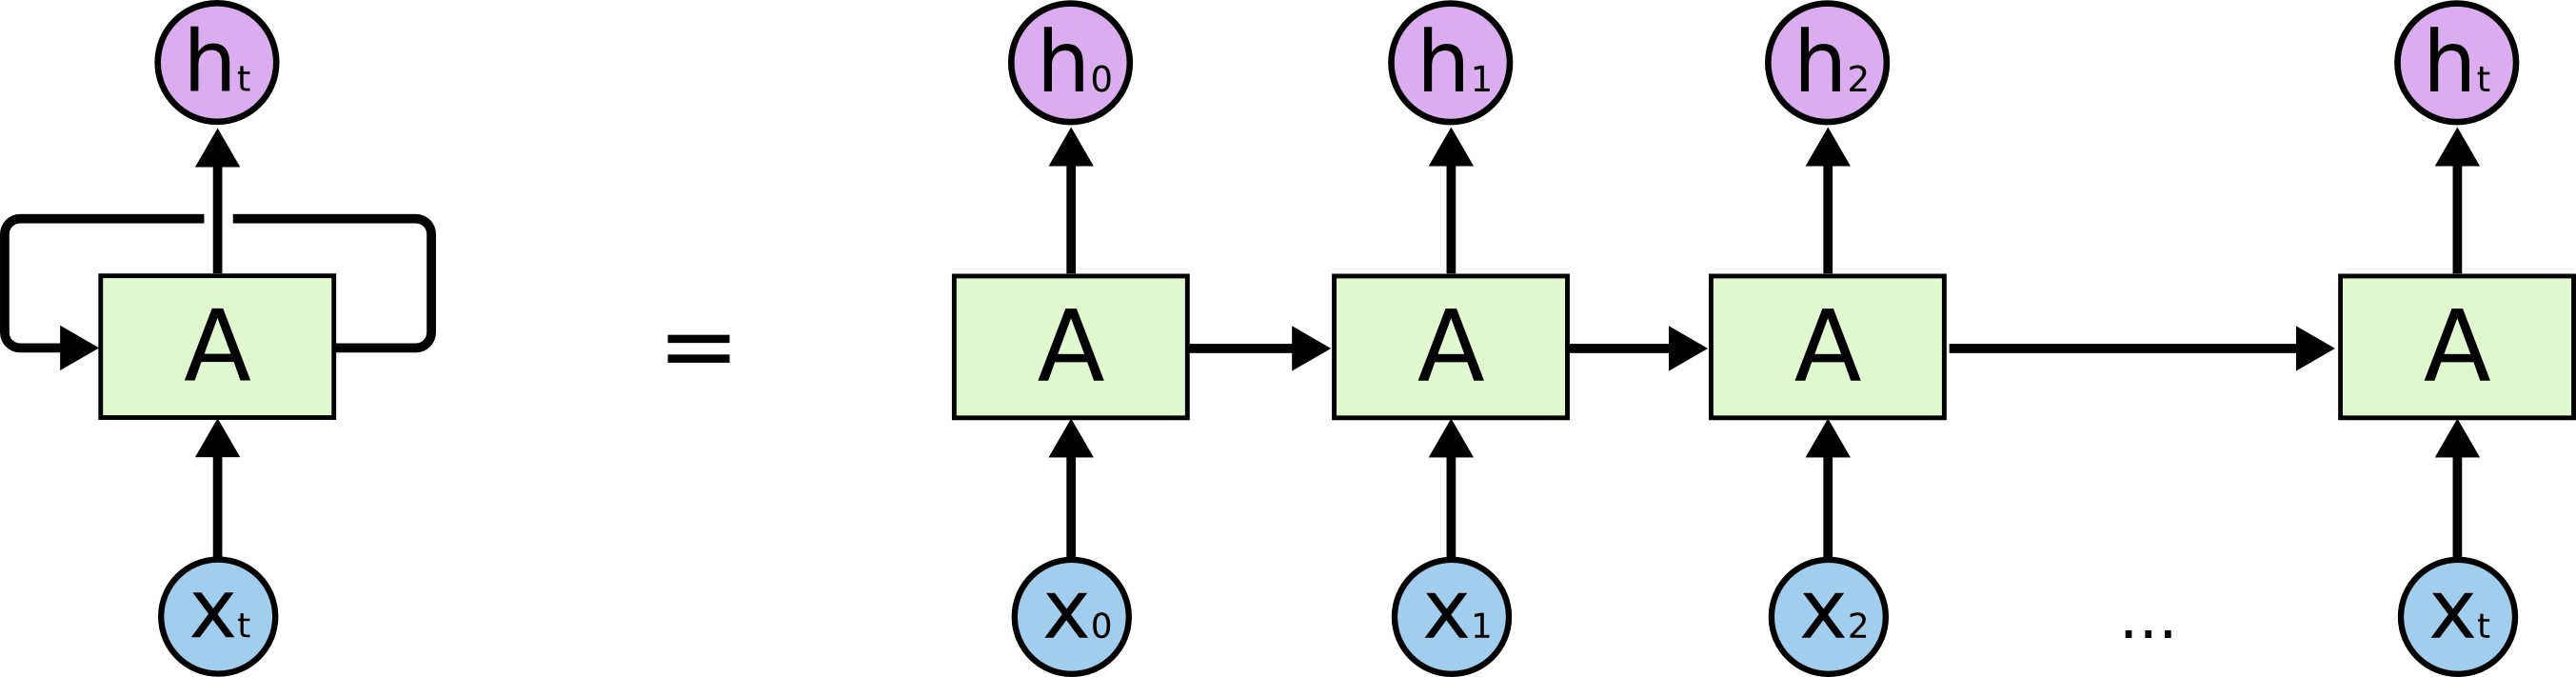
\includegraphics[width=1.0\linewidth]{img/RNN-unrolled.png}}
    \end{center}
	\caption{Znázornění RNN -- $x_t$ je vstup, $A$ zastupuje vnitřní chování RNN a $h_t$ je skrytý stav. Rozdílem oproti běžné dopředné neuronové síti je zpětná smyčka a skrytý stav. Pravá část obrázku ukazuje pro lepší představu místo zpětné smyčky rozbalenou strukturu přes jednotlivé časy $t$. Intuitivně se pak dá odhadnout, že RNN umí dobře pracovat s~podobnými strukturami jako jsou sekvence a seznamy. Obrázek převzat z~\cite{understandingLSTM}.}	
	\label{img:rnn}
\end{figure}

Rovnice RNN pro výpočet vnitřního stavu:
\begin{align}\label{figure:rnn}
  h_t = \begin{cases}
          f(W_{xh}x_t + W_{hh}h_{t-1} + b_h) & \mbox{pokud t $\geq$ 1}, \\
          0 & \mbox{jinak}.
        \end{cases}
\end{align}


$W_{xh}$ znázorňuje váhy pro aktuální vstup, $W_{hh}$ jsou váhy pro skrytý stav z~minulého kroku a $b_h$ je bias. Funkce $f$ z~rovnice \ref{figure:rnn} je nelineární funkcí a nejčastěji se používá jedna z~funkcí \emph{step}, \emph{sigmoida}, \emph{tanh} nebo \emph{relu} (obrázek \ref{img:functions}).

\begin{figure}[H]
    \begin{center}
            \tmpframe{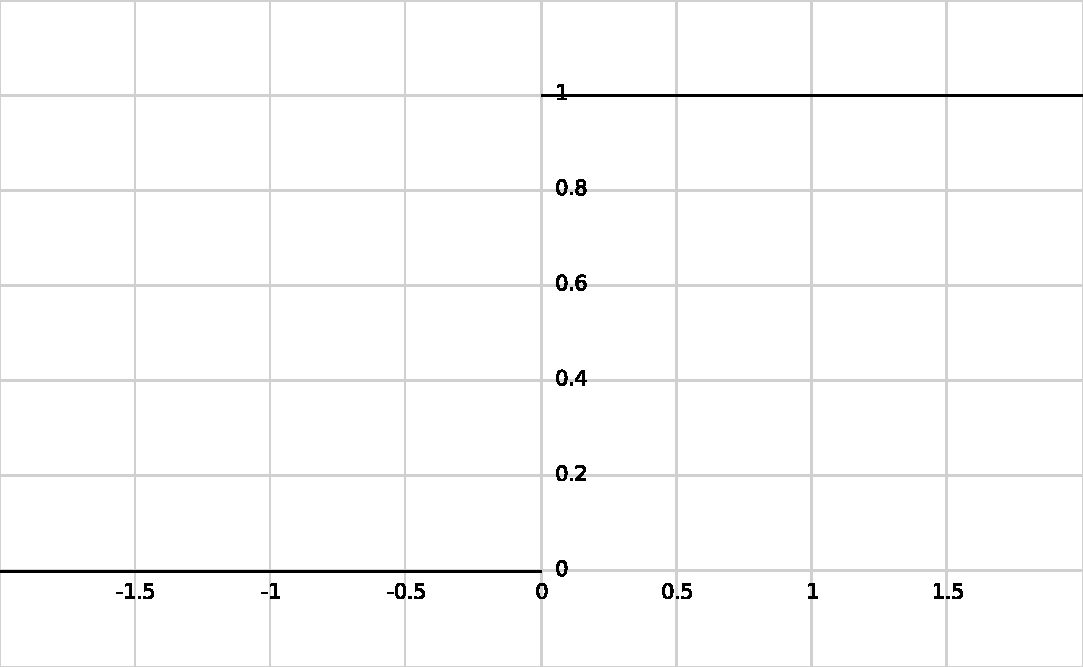
\includegraphics[width=0.45\linewidth]{img/step.pdf}}
            \tmpframe{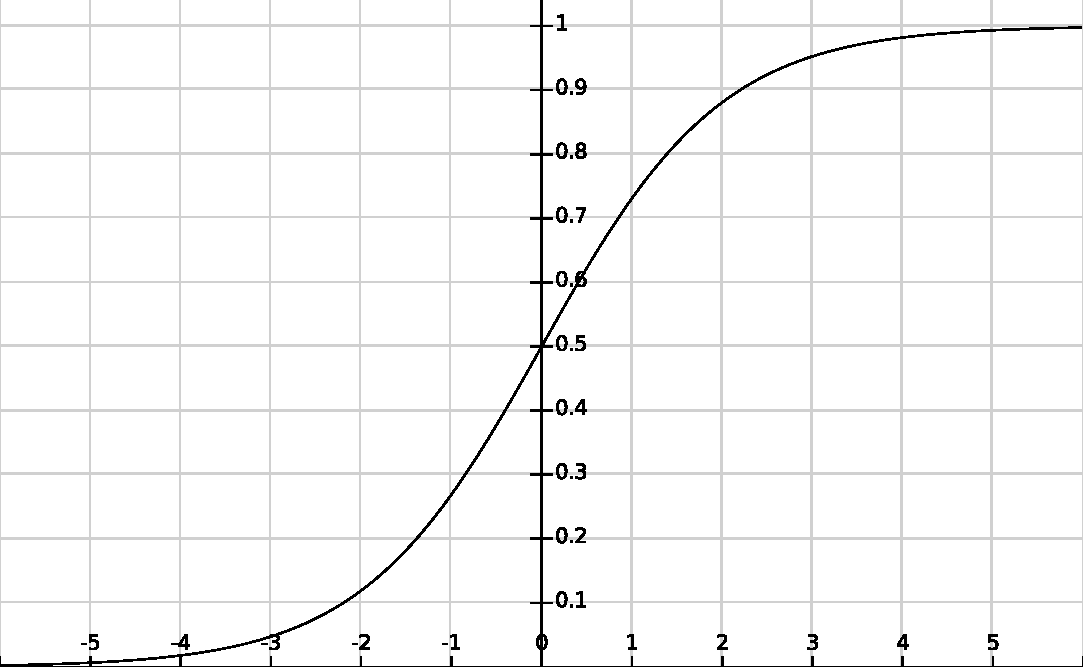
\includegraphics[width=0.45\linewidth]{img/sigmoid.pdf}}
            \tmpframe{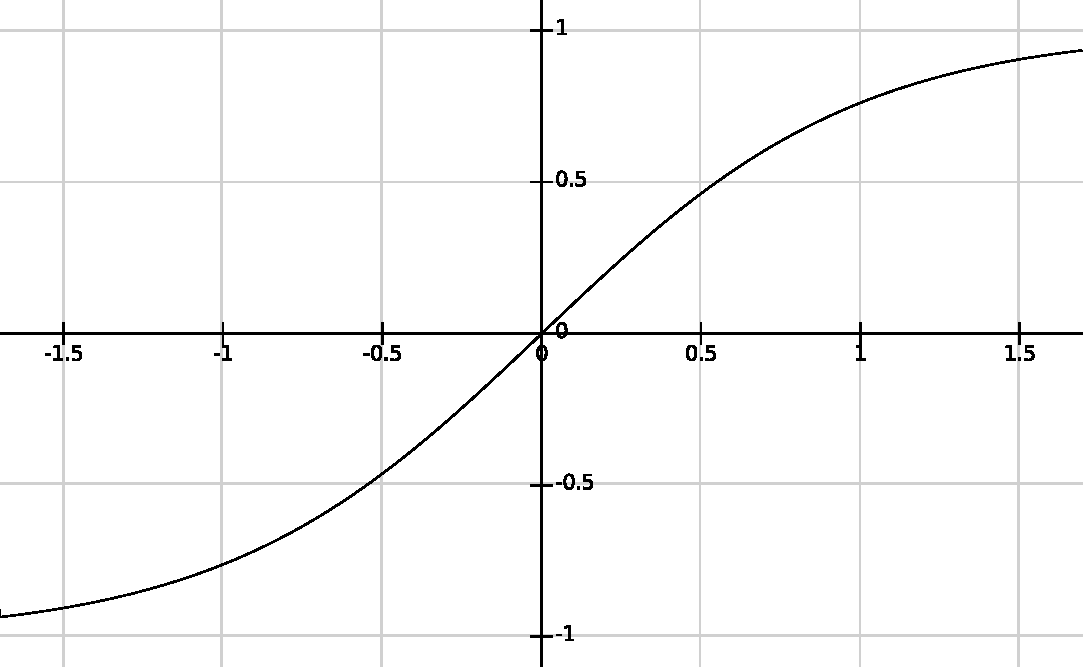
\includegraphics[width=0.45\linewidth]{img/tanh.pdf}}
            \tmpframe{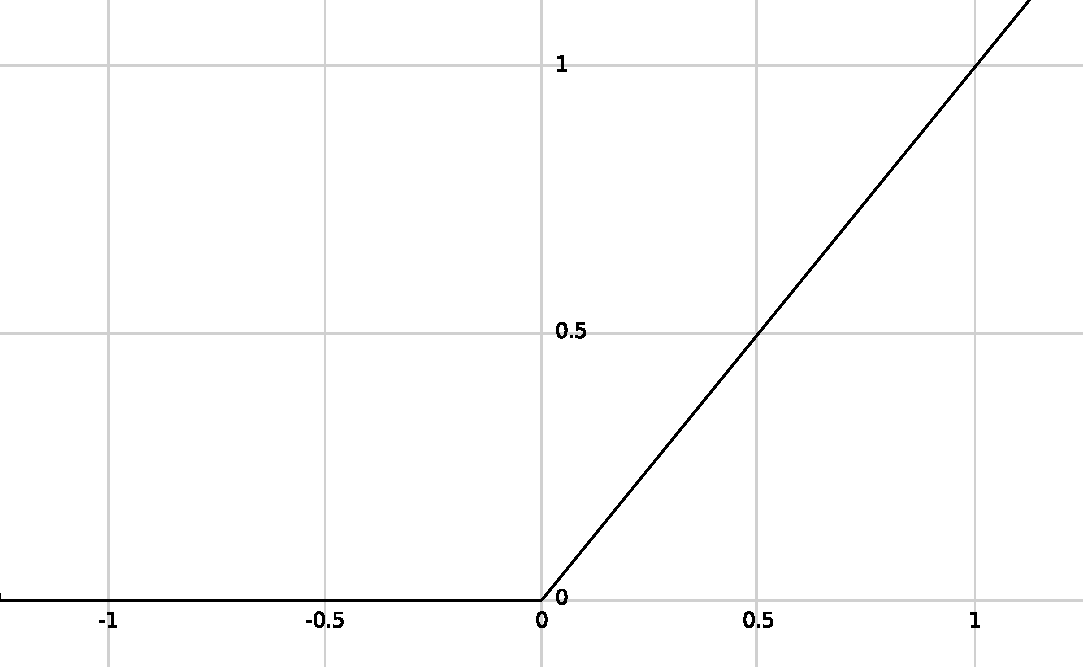
\includegraphics[width=0.45\linewidth]{img/relu.pdf}}
    \end{center}
	\caption{Nelineární funkce $step$, $sigmoida$, $tanh$ a $relu$.}
	\label{img:functions}
\end{figure}

Rovnice pro RNN jazykový model jsou následující:

\begin{align}
  m_{t}&=M_{e_{t-1}}\label{figure:lastContext} \\
  h_{t}&=RNN(m_t, h_{t-1}) \label{figure:rnnSimple} \\
  s_{t}&=W_{hs}h_t + b_s \label{figure:rnnSt} \\
  p_{t}&=softmax(s_t) \label{figure:rnnSoftmax}
\end{align}


kde \ref{figure:lastContext} je aktuální kontext, \ref{figure:rnnSimple} je zjednodušený přepis rovnice RNN (\ref{figure:rnn}) a rovnice \ref{figure:rnnSoftmax} je funkce softmax, která je podrobněji popsána v~\ref{figure:softmax}. Softmax vezme všechny hodnoty skóre pro jednotlivá slova a transformuje je do pravděpodobnostního rozdělení $p_t$. Díky tomu pak lze již snadno určit, které slovo bude vygenerováno s~největší pravděpodobností.


\begin{align}\label{figure:softmax}
  p_t(y)={\frac {e^{p_{t}(y)}}{\sum _{k=1}^{K}e^{p_{t_{k}}}}}
\end{align}
\\


Protože vektor $m$ z~rovnice \ref{figure:lastContext} je konkatenací všech předchozích slov (a tedy je to aktuální kontext), model se může naučit kombinaci různých vlastností napříč několika různými slovy z~kontextu. V~sekci \ref{subsection:loglinear} byl jako problém uveden příklad \uv{Farmář jí steak} a \uv{Kráva jí steak}, kde druhá věta nedává smysl. Při použití RNN by se pro kontext $M_f$  \{farmář, jí\} mohla naučit jedna z~jednotek skryté vrstvy $h$ rozpoznat vlastnost "věci, které jí farmář" a správně se aktivovat a pak nabízet slova jako \uv{steak} nebo \uv{brambory}. Zatímco pro kontext $M_k$ \{kráva, jí\} by se naučila zase jiná jednotka. RNN je tedy schopná zachytit tyto vzdálenější závislosti. Základní verze RNN je však schopná zachytit závislosti jen do určité vzdálenosti viz \ref{subsection:gradient}.


\subsection{Trénování} \label{subsection:training}
Cílem trénování sítě je nalézt takové parametry $\theta$ (kombinace vah $W$ a biasu $b$), aby se minimalizovala hodnota takzvané \emph{loss funkce}. Loss funkce vyjadřuje jak moc špatně výstupy sítě odpovídají datům, na kterých se síť trénuje. Průchod sítí a následné vypočítání loss funkce se nazývá \emph{dopřednou propagací}.


%\todo{jakej pouzit vzorec}
%\begin{align}\label{figure:loss}
%  a
%\end{align}

K~optimalizaci parametrů pro nalezení minima loss funkce se používá \emph{zpětná propagace}. Vypočte se přírůstek pro každý parametr tak, aby síť s~novými váhami o~něco lépe pracovala a loss funkce se snížila. Existuje více různých metod optimalizace pro tento výpočet podrobně popsaných v~práci \cite{gradientDescent}.

Úprava parametrů může probíhat po každém jednom průchodu dat (jedné sekevence) sítí. Takovýto přístup se nazývá \textbf{online} učení. Dalším přístupem je \textbf{učení po dávkách}. V~takovém to případě probíhá přepočet parametrů až po průchodu přes $n$ sekvencí. Toto číslo $n$ se nazývá \textbf{batch size}, tedy počet dat  v~jedné dávce.

%\todo{epoch, batchsize....loss, back propagation (over time)}
%\todo{z tutorialu, sekce 6.5 strana 35..nejak popsat batch, minibatch, online batch, sentence padding a masking}
%
%\todo{trénování rnn, back propagation through time, have difficulties (\url{http://proceedings.mlr.press/v28/pascanu13.pdf}) learning long term dependencies}
%\todo{loss computing}
%\todo{gradient computing}
%
%Gradient descent methods
%\begin{itemize}
%  \item a
%\end{itemize}
%
%\url{http://ruder.io/optimizing-gradient-descent/index.html#stochasticgradientdescent}
%\todo{jak prelozit gradient descent? popsat co to je, ke cemu to je a pak vypsat ty jednotlivy metody a trochu je popsat}
%\url{https://arxiv.org/abs/1609.04747}


\subsection{Mizející a explodující gradient} \label{subsection:gradient}
RNN jsou oproti základním neuronovým sítím schopné zachytit různé závislosti mezi slovy na delší vzdálenosti. I~tato schopnost je však velmi limitovaná. Hlavními zdroji problémů jsou \textbf{mizející a explodující gradient} (článek \cite{gradientProblems}).

%\todo{patrne v nejake predchozi casti zhruba popsat LOSS, BACKPROPAGATION aby se tady na to pak dalo navazat} v sekci \ref{subsection:training}

Při průběhu učení RNN průběžně vznikají predikce a počítá se \emph{loss} funkce. Následně je potřeba zpětně zpropagovat tuto hodnotu přes všechny (časové) kroky sítě (Back propagation through time -- BPTT). Pokud však není gradient rovný 1, tak se v~každém zpětném kroku buďto zmenší a tím pádem se blíží k~nule, nebo se naopak zvětší a blíží se k~nekonečnu. Ve výsledku je tak gradient buďto příliš malý a nemá tak žádný efekt na úpravu vah, nebo jimi pohne příliš a tak zaviní špatné učení se sítě.

Jako možné řešení těchto problémů vznikla varianta rekurentní sítě LSTM (sekce \ref{section:LSTM}).


\subsection{LSTM}\label{section:LSTM}
Long short term memory, dále LSTM, (původní článek \cite{LSTM} a varianta LSTM s~forget gate z~článku \cite{forgetLSTM}, která je zde použitá), neboli dlouhá krátkodobá paměť, je varianta RNN navržená jako řešení problémů mizejícího/explodujícího gradientu a vzdálených závislostí.

Stejně jako základní RNN (sekce \ref{section:rnn}) se dá LSTM představit jako opakující se modul v~řetězové struktuře (viz obrázek \ref{img:rnn}). Rozdíl je ve vnitřku modulu $A$. Zatímco RNN používá pouze jednu nelineární funkci (rovnice \ref{figure:rnn}), struktura LSTM je složitější (obrázek \ref{img:LSTM} a následující rovnice).

\begin{align}
    u_{t}&=tanh(W_{xu}x_t + W_{hu}h_{t-1} + b_u) \label{figure:update} \\
    f_{t}&=\sigma(W_{xf}x_{t}+W_{hf}h_{t-1}+b_{f}) \label{figure:forgetGate} \\
    i_{t}&=\sigma(W_{xi}x_{t}+W_{hi}h_{t-1}+b_{i}) \label{figure:inputGate} \\
    o_{t}&=\sigma(W_{xo}x_{t}+W_{ho}h_{t-1}+b_{o}) \label{figure:outputGate} \\
    c_{t}&=i_{t}\odot u_{t}+f_{t}\odot c_{t-1}\label{figure:memoryCell} \\
    h_{t}&=o_{t}\odot tanh(c_{t}) \label{figure:hiddenState}
\end{align}

RNN má pouze skrytý stav $h$. LSTM má navíc ještě paměťovou buňku $c$ (rovnice \ref{figure:memoryCell}). Protože gradient této buňky je roven jedné, netrpí tak LSTM problémy ze sekce \ref{subsection:gradient} a mohou tak v~ní být zachyceny i vzdálené závislosti.

Rovnice \ref{figure:update} je update funkcí a je ekvivalentem rovnice \ref{figure:rnn} z~RNN.
Dále LSTM obsahuje tři různé \textbf{brány}. \textbf{Zapomínací}, \textbf{vstupní} a \textbf{výstupní}. Tyto brány určují a kontrolují, co se nachází v~paměti $c_t$.

Nejdříve se LSTM rozhodne, jaké informace se vyhodí z~paměti. K~tomuto slouží již zmíněná zapomínací brána neboli forget gate (rovnice \ref{figure:forgetGate}). Například v~případě, že síť narazí na vstupu na podstatné jméno, mohla by chtít zapomenout rod posledního podstatného jména, který by si mohla uchovávat pro správné generování sloves v~minulém čase.

Dalším krokem je vyhodnocení toho, co se má přidat do paměti. Nejdříve vstupní brána neboli input gate (rovnice \ref{figure:inputGate}) rozhodne, které hodnoty se změní nebo přidají. V~návaznosti na minulý příklad by síť mohla chtít uložit aktuální rod nalezeného podstatného jména. Update funkce (rovnice \ref{figure:update}) vyhodnotí, jaké hodnoty se mají přidat.

Následuje aktualizace paměti $c_t$ (rovnice \ref{figure:memoryCell}). V~kontextu příkladu by se zahodil rod, jak určila zapomínací brána a uložil se nový rod podle vstupní brány.

Posledním krokem je určení toho co vydá LSTM na výstupu (skrytý stav $h_t$). Výstupní brána určí, co z~paměti $c_t$ má projít (rovnice \ref{figure:outputGate}) a v~rovnici \ref{figure:hiddenState} se získá výsledek.

Pravděpodobnosti jazykového modelu se získají rovnicí:
\begin{align}
    p_t = softmax(W_{hs}h_{t} + b_{s})
\end{align}


\begin{figure}[H]
    \begin{center}
            \tmpframe{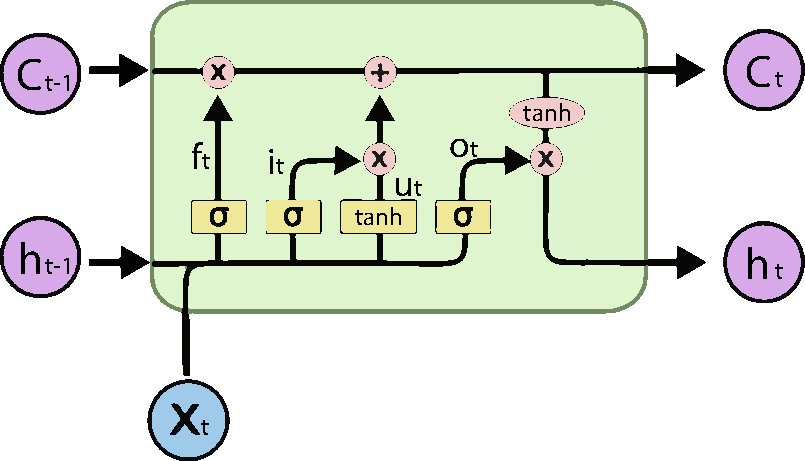
\includegraphics[width=0.8\linewidth]{img/LSTM.pdf}}
    \end{center}
	\caption{Jeden časový úsek LSTM kde $h$ je skrytý stav, $c$ je paměťová buňka a $x$ je vstup. Vnitřní struktura koresponduje s~rovnicemi \ref{figure:update} až \ref{figure:hiddenState}. Obrázek převzat z~\cite{understandingLSTM}, upraven.}
	\label{img:LSTM}
\end{figure}



\subsection{GRU}\label{section:GRU}
LSTM z~minulé sekce je dobrým řešením pro problémy ze sekce \ref{subsection:gradient}. Má však dosti komplikovanou strukturu a tím pádem jsou i vyšší nároky na výpočetní výkon. To podnítilo vznik další varianty RNN --- GRU, neboli gated recurrent unit (článek \cite{GRU}). GRU je o~něco jednodušší, a proto je to vhodnější varianta pro úsporu výkonu.

\begin{align}
    r_{t}&=\sigma(W_{xr}x_{t}+W_{hr}h_{t-1}+b_{r}) \label{figure:resetGate} \\
    z_{t}&=\sigma(W_{xz}x_{t}+W_{hz}h_{t-1}+b_{z}) \label{figure:updateGate} \\
    \tilde{h}_{t}&=tanh(W_{xh}x_t + W_{hh}(r_t \odot h_{t-1}) + b_h) \label{figure:candidate} \\
    h_{t}&=(1 - z_t)h_{t-1} + z_{t}\tilde{h}_{t}) \label{figure:hiddenStateGru}
\end{align}

GRU má pouze dvě brány a skrytý stav $h$. Nový stav se počítá v~rovnici \ref{figure:hiddenStateGru} interpolací mezi minulým stavem $h_{t-1}$ a kandidátem na nový stav $\tilde{h}_{t}$ upravený hodnotou \textbf{update} brány (rovnice \ref{figure:updateGate}). Kandidát se získá v~rovnici \ref{figure:candidate}, která je podobná update funkci z~RNN (rovnice \ref{figure:rnn}), ale je upravena hodnotou \textbf{resetovací} brány (rovnice \ref{figure:resetGate}). Struktura je zobrazená na obrázku \ref{img:GRU}.


\begin{figure}[H]
    \begin{center}
            \tmpframe{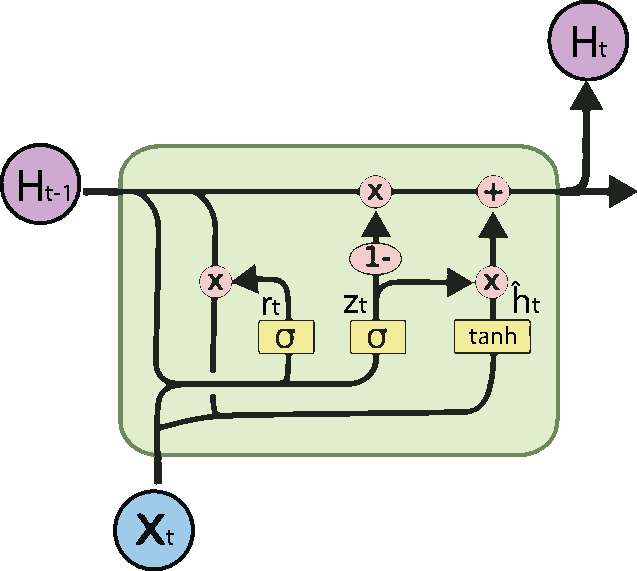
\includegraphics[width=0.65\linewidth]{img/GRU.pdf}}
    \end{center}
	\caption{Jeden časový úsek GRU, kde $h$ je skrytý stav a $x$ je vstup. Vnitřní struktura koresponduje s~rovnicemi \ref{figure:resetGate} až \ref{figure:hiddenStateGru}. Obrázek převzat z~\cite{understandingLSTM}, upraven.}
	\label{img:GRU}
\end{figure}

\section{Seq2seq model s~architekturou enkodér-dekodér} \label{section:encoderdecoder}
V~předchozích sekcích se práce zabývá rekurentními neuronovými sítěmi a jazykovými modely na nich postavenými. V~této sekci bude popsáno, jak tyto sítě vzít a poskládat je vhodným způsobem pro překlad vět. Sekce vychází z~práce \cite{nmtTutorial}.

\textbf{Seq2seq} (článek \cite{seq2seq}) neboli sequence to sequence je způsob překladu po celých větách. Jde o~modelování pravděpodobnosti $P(E|F)$, tedy pravděpodobnosti výstupu $E$ na základě vstupu $F$ (obrázek \ref{figure:seqProbability}).

\begin{figure}[H]
    \begin{center}
        \setlength{\fboxsep}{8pt}
        \fbox{$W_{in}$ = \uv{Ahoj světe}}
        $\Longrightarrow$
        \fbox{$W_{out}$ = \uv{Hello world}}
        \\ \vspace{5mm}
        $P(W_{out}|W_{in})$
    \end{center}
	\caption{Seq2seq modeluje pravděpodobnost $P(W_{out}|W_{in})$. Znamená to, že se naučí předpovídat větu $W_{out}$ na základě věty $W_{in}$ a tím pádem překládat.}
	\label{figure:seqProbability}
\end{figure}

Pro tento druh překladu celých vět za pomocí rekurentních neuronových sítí se používá model s~architekturou \textbf{enkodér-dekodér}. Enkodér i dekodér jsou RNN modely. Enkodér dostane na vstupu větu určenou pro překlad a převede ji (enkóduje) do vektoru reálných čísel. Tento výsledný skrytý stav, takzvaný myšlenkový vektor, vyjadřuje význam dané věty. Dekodér inicializovaný tímto stavem generuje (dekóduje) z~myšlenkového vektoru přeloženou větu. Díky tomu, že dekodér generuje na základě stavu, kterým byl inicializován, není nijak vázaný na délku původní věty a přeložená věta tak může být jinak dlouhá.


\begin{align}
    m^{(f)}_{t}&=M^{(f)}_{f_t}\label{figure:encoderEmb} \\
    h^{f}_{t}&=\begin{cases}
                    RNN^{(f)}(m^{(f)}_{t},h^{(f)}_{t-1}) & \mbox{pokud t $\geq$ 1},\label{figure:encoderState} \\
                    0 & \mbox{jinak}.
                \end{cases}\\
    m^{(e)}_{t}&=M^{(e)}_{e_{t-1}}\label{figure:decoderEmb} \\
    h^{e}_{t}&=\begin{cases}
                    RNN^{(e)}(m^{(e)}_{t},h^{(e)}_{t-1}) & \mbox{pokud t $\geq$ 1},\\
                    h^{f}_{|F|} & \mbox{jinak}.
                \end{cases}\label{figure:decoderState} \\
    p^{(e)}_{t}&=\mbox{softmax}(W_{hs}h^{(e)}_{t} + b_{s}) \label{figure:resultSoftmax}
\end{align}


Pro každé slovo v~čase $t$ ze vstupní sequence $F$ se vyhledá jeho embedding (rovnice \ref{figure:encoderEmb}). Následně se v~rovnici \ref{figure:encoderState} spočítá skrytý stav enkodéru. Po projití přes celou vstupní větu by měly uvnitř být uloženy všechny informace potřebné pro inicializaci dekodéru. I~pro dekodér se nejprve vyhledá pro vstupní slovo jeho embedding (rovnice \ref{figure:decoderEmb}). Použité slovo není z~času $t$, ale z~času $t-1$, protože dekodér generuje následující slovo vždy na základě předchozího. V~čase $t_0$ se jako vstupní slovo používá \textbf{startovací} symbol <s>. Rovnice pro výpočet skrytého stavu dekodéru (\ref{figure:decoderState}) je prakticky stejná jak u~enkodéru. Pouze v~čase $t_0$ se použije koncový stav enkodéru jako inicializace ze které může dekodér vycházet při překladu -- ve vnitřním stavu je zachycen význam věty, kterou má přeložit. Pravděpodobnostní rozdělení se pak jako u~všech jazykových modelů spočítá pomocí funkce \emph{softmax} (rovnice \ref{figure:resultSoftmax}).


\subsection{Průběh trénování a generování}

Cílem jazykového modelu je předpovídat následující slovo ve větě. Při trénování se nejprve do enkodéru pošle výchozí věta, aby se získal inicializační stav pro dekodér. Do dekodéru, inicializovaného získaným stavem, se nejprve pošle \textbf{startovací} symbol. Startovací symbol dekodéru říká, že má začít překládat. Při trénování se mu pak následně posílají korektní další slova referenčního překladu, aby se zrychlilo učení. Tato metoda se nazývá \uv{teacher forcing}\label{teacherForcing} (\cite{teacherForcing}). Proces je znázorněný na obrázku \ref{img:seq2seq}. Po naučení modelu se ve fázi generování do dekodéru posílají slova, která již sám vygeneroval (obrázek \ref{img:inference}). Dekodér generuje tak dlouho, dokud nenarazí na \textbf{koncový} symbol, kterým je v~době trénování zakončená každá věta. Ve skutečnosti však výstupem dekodéru není přímo slovo, ale rozdělení pravděpodobnosti přes všechna slova cílového slovníku získaného funkcí \emph{softmax} v~rovnici \ref{figure:resultSoftmax}. Je několik možností jak z~tohoto rozdělení vybrat konkrétní slovo:

\begin{description}
  \item[Náhodný výběr:] Z~rozdělení pravděpodobnosti $P(E|F)$ se slovo vybere náhodně.
  \item[Chamtivý výběr:] Chamtivý (greedy) výběr spočívá ve výběru slova, které získalo největší pravděpodobnost -- argmax($P(E|F)$).
  \item[Paprskové prohledávání:]\label{decsription:beamsearch} Z~anglického beam search, paprskové prohledávání najde $n$ výstupů s~největší pravděpodobností $P(E|F)$, které drží jako $n$ možných výsledků neboli hypotéz. V~každém kroku $t$ se každá hypotéza rozšíří o~další slovo a ze všech aktuálních hypotéz se zase vybere $n$ nejslibnějších. Až jsou všechny hypotézy ukončeny koncovým symbolem <eos>, vybere se z~nich ta s~největší pravděpodobností, jako výsledek.
\end{description}


\begin{figure}[H]
    \begin{center}
            \tmpframe{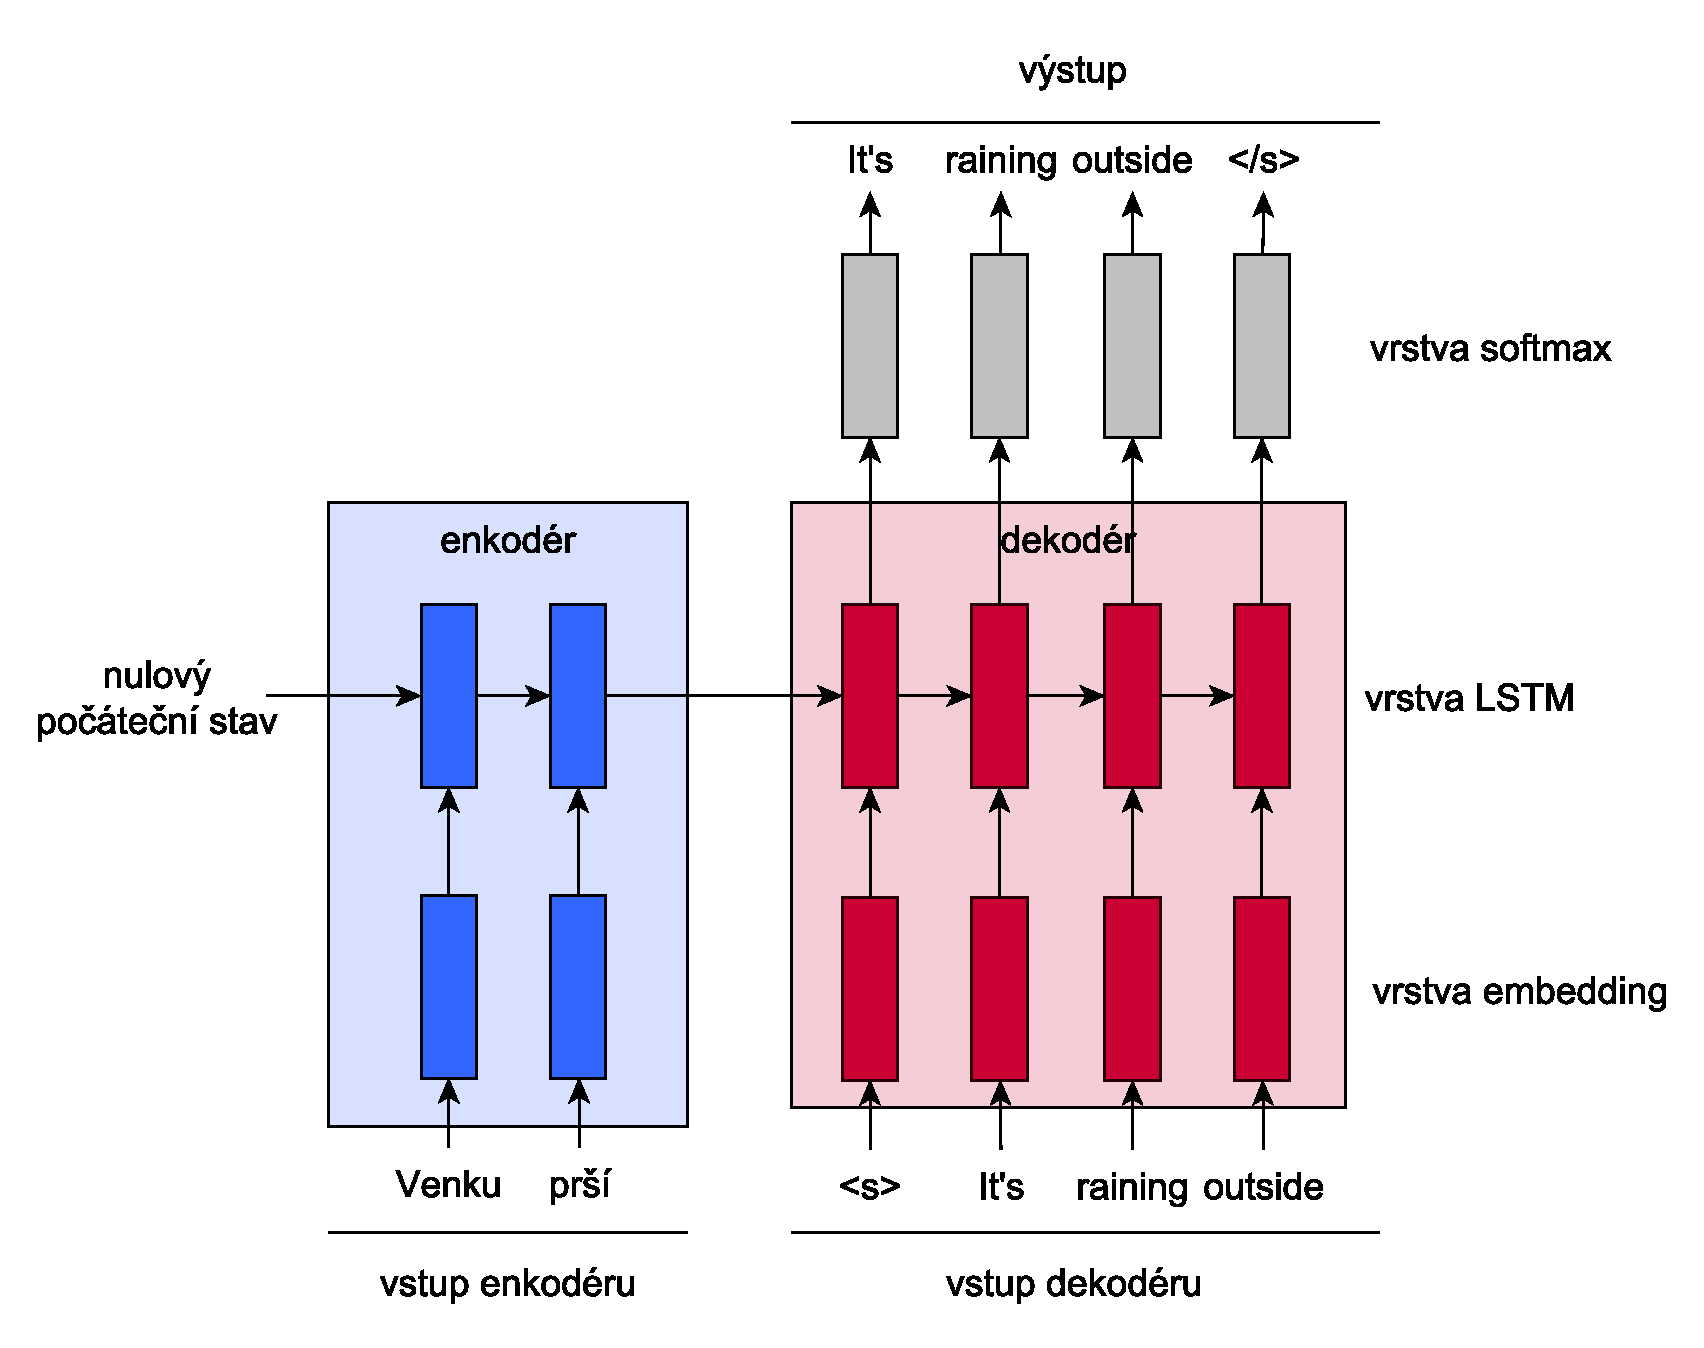
\includegraphics[width=1\linewidth]{img/graphs/seq2seq.pdf}}
    \end{center}
	\caption{Architektura enkodér-dekodér. Enkodér obdrží větu na vstupu a vytvoří inicializační stav pro dekodér (\uv{myšlenkový vektor}). Tímto vektorem je inicializován počáteční stav dekodéru. Ten v~době trénování dostává na vstupu správně přeloženou větu (teacher forcing) a v~době generování na vstup dostává slova, která sám vygeneroval. Konečný výstup se získá pomocí vrstvy softmax.}
	\label{img:seq2seq}
\end{figure}

\begin{figure}[H]
    \begin{center}
            \tmpframe{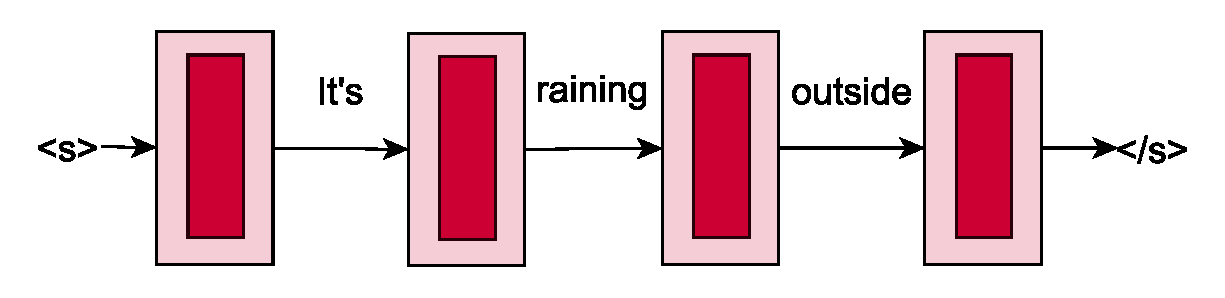
\includegraphics[width=0.8\linewidth]{img/graphs/inference.pdf}}
    \end{center}
	\caption{Ukázka práce dekodéru v~době predikce překladu (inference). Na vstup jako první přichází startovací symbol <s>. Následně v~každém dalším kroku na vstup dekodéru dostane svůj vlastní výstup z~kroku minulého. Takto generuje tak dlouho, dokud nenarazí na koncový symbol </s>.}
	\label{img:inference}
\end{figure}

\subsection{Metody optimalizace} \label{subsection:optimization} V~této sekci jsou popsány způsoby jakými lze zlepšit výkon seq2seq modelu.

\begin{description}
  \item[Převrácení vstupu:] \label{desc:revert} Článek \cite{seq2seq} udává, že výrazným způsobem pomůže, když se slova ve vstupní sekvenci převrátí a do enkodéru  se věta předává pozpátku. Pravděpodobně je to díky tomu, že závislosti, které by běžně byly vzdálené -- typicky poslední slovo ve vstupní větě a jeho přeložená varianta v~přeložené větě -- jsou si takhle blíž. Díky tomu se může model snáz a rychleji učit.
  \item[Obousměrný enkodér:] \label{desc:biriectional} Zatímco převrácení vstupu pomůže jen pokud jsou slova ve větách překládaných jazyků na podobných místech (což není pravda napříč všemi jazyky), tato varianta je spolehlivější. Místo jednoho enkodéru se použijí dva a každý z~nich projde větu jedním směrem. Jejich výsledky se pak spojí do jednoho skrytého stavu $h$, kterým se již běžně inicializuje dekodér.
  \item[Hloubka sítí:] Enkodér i dekodér jsou RNN a mohou obsahovat více skrytých vrstev (ať již základní varianty, LSTM nebo GRU). Článek \cite{googleBridgingGap} udává, že více vrstev může do určité hloubky pomoci. V~práci jich vědci použili 8 jak pro enkodér tak dekodér. Při použití většího množství již má model problém se úspěšně učit.
  \item[Reziduální propojení:] \label{residuals} V~práci \cite{googleBridgingGap} doporučují při použití více vrstev LSTM použít takzvané reziduální propojení nebo zapojení mezi vrstvami. Podle jejich experimentů při použití většího počtu vrstev a běžném zapojení začne být učení pomalé a složité. Řešením je použití reziduálního propojení vrstev. Běžně by do vrstvy $LSTM_0$ vstupoval vstup $x_0$ a do vrstvy $LSTM_1$ vstup $x_1$, který je výstupem vrstvy $LSTM_0$. Při reziduálním propojení vstupuje do každé následující vrstvy výstup z~vrstvy minulé sečtený dohromady se vstupem minulé vrstvy. Tedy do $LSTM_1$ vchází $x_1+x_0$ (obrázek \ref{img:residuals}).
  \item[Dropout:] \label{desc:dropout} Při trénování neuronových sítí může dojít k~přetrénování -- síť se naučí podávat správné výsledky pro trénovací data, ale bude mít malou nebo žádnou schopnost generalizce, tedy nebude fungovat nad jinými než trénovacími daty. Dropout (\cite{dropout}), je regulační metoda používaná k~předejití přetrénovaní. Metoda spočívá v~náhodném zahazování výsledků některých neuronů v~době trénovaní, čímž se snaží síť udělat více robustní, protože se síť nemůže spoléhat na výstupy konkrétních neuronů.

\end{description}

\begin{figure}[H]
    \begin{center}
            \tmpframe{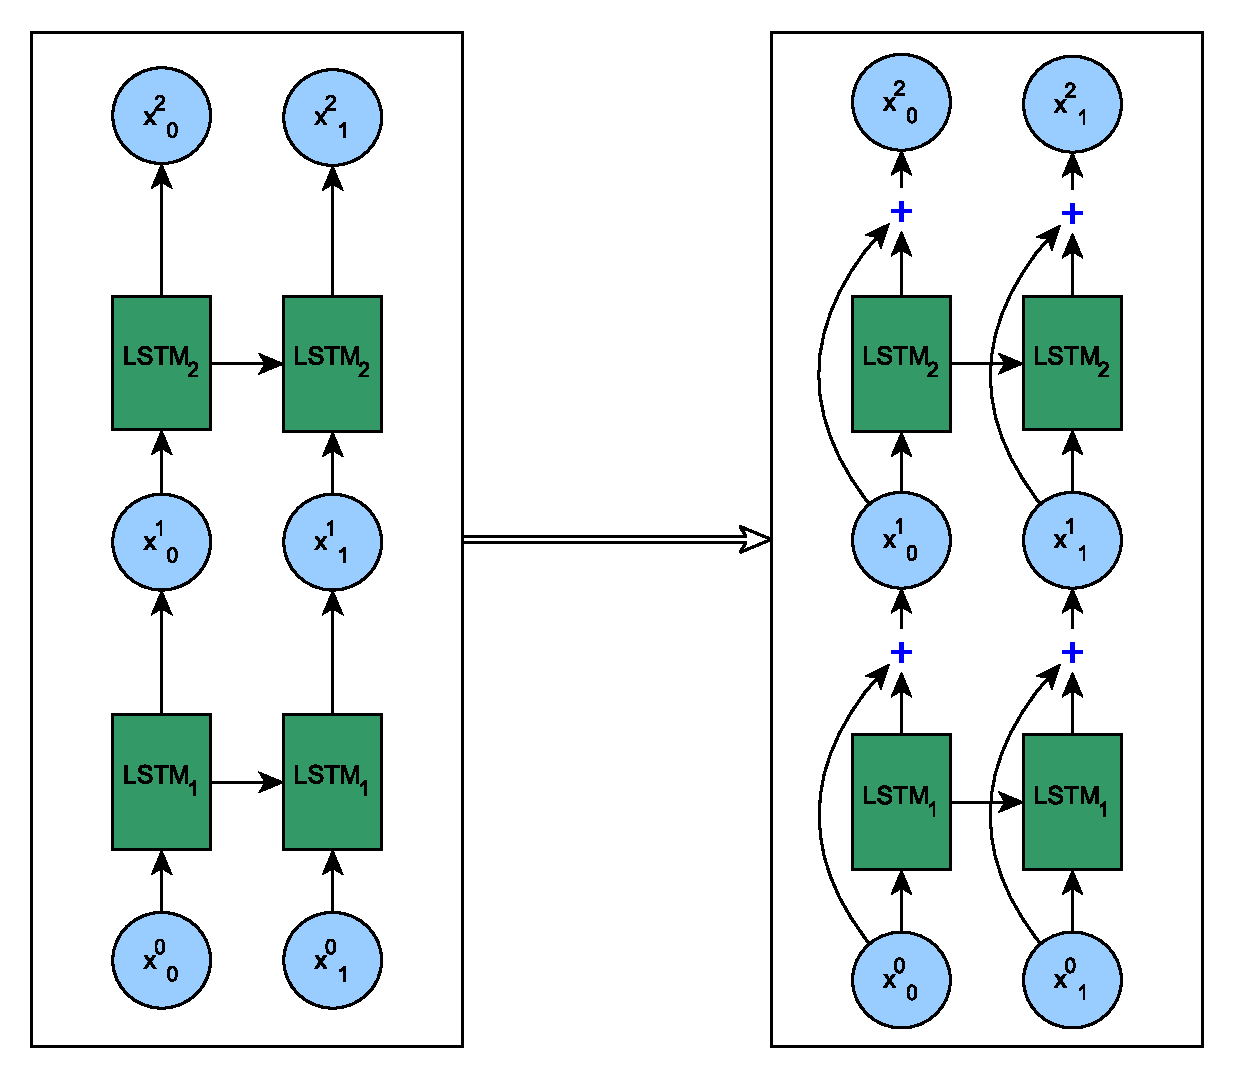
\includegraphics[width=0.9\linewidth]{img/graphs/residuals.pdf}}
    \end{center}
	\caption{Rozdíl mezi normálním a reziduálním propojení pro zlepšení učení více vrstvých LSTM. Levý obrázek znázorňuje běžné zapojení, zatímco na pravém je ukázka reziduálního propojení. Do každé (kromě první) vrstvy $LSTM_i$ vstupuje součet výstupu vrstvy minulé $x_i$ sečtený se vstupem minulé vrstvy $x_{i-1}$.}
	\label{img:residuals}
\end{figure}


\subsection{Překlad mezi více jazyky s~jedním modelem} \label{section:multilingual}
Doposud udávané informace se týkaly překladu z~jednoho jazyka do druhého, tedy existují páry vět mezi dvěmi jazyky, enkodér se natrénuje na větách ve zdrojovém jazyce a dekodér se naučí překládat pomocí vět v~cílovém jazyce.

Google ve své práci \cite{googleMultiLingual} ukazuje, že se stejným enkodér-dekodér modelem lze bez jeho úprav překládat mezi několika jazyky.
Jediným rozdílem je přidání speciálního tokenu před zdrojové věty. Tento token udává do jakého jazyka se má daná věta překládat (znázorněno na obrázku \ref{figure:multiLingDataset}). V~práci se používá slovník wordpieces (\ref{subsection:subwords}) natrénovaný a sdílený přes všechny použité jazyky.


\begin{figure}[H]
    \begin{center}
        \begin{tabular}{| >{\centering\arraybackslash}p{0.3\linewidth} |}
          \hline
          Ahoj světe. \\
          Venku prší. \\
          \hspace{1mm} \vdots \\
          Farmář jí steak. \\
          \hline
        \end{tabular}
        $\Longleftrightarrow$
        \begin{tabular}{| >{\centering\arraybackslash}p{0.3\linewidth} |}
          \hline
          Hello world. \\
          It's raining outside. \\
          \hspace{1mm} \vdots \\
          Farmer eats steak. \\
          \hline
        \end{tabular}
    \end{center}
    \begin{minipage}[t]{1\linewidth}
        \centering
        \subcaption{Příklad párů vět mezi dvěmi jazyky.}\label{subcap:singlePair}
    \end{minipage}%

    \begin{center}
        \begin{tabular}{| >{\centering\arraybackslash}p{0.3\linewidth} |}
          \hline
          <en> Ahoj světe. \\
          <cs> Hello world. \\
          \hspace{1mm} \vdots \\
          <fr> Hola Mundo. \\
          \hline
        \end{tabular}
        $\Longleftrightarrow$
        \begin{tabular}{| >{\centering\arraybackslash}p{0.3\linewidth} |}
          \hline
          Hello world. \\
          Ahoj světe. \\
          \hspace{1mm} \vdots \\
          Bonjour monde \\
          \hline
        \end{tabular}
    \end{center}
    \begin{minipage}[t]{1\linewidth}
        \centering
        \subcaption{Příklad párů vět se speciálním tokenem, který odlišuje do jakého jazyka má být věta přeložena. Model může překládat z~vícero do vícero jazyků.}\label{subcap:multiLingual}
    \end{minipage}%

	\caption{Obrázek ukazuje rozdíl mezi páry vět použitými při běžném překladu mezi dvěmi jazyky (\ref{subcap:singlePair}) a při použití stejného modelu pro překlad mezi více jazyky (\ref{subcap:multiLingual}). Je potřeba přidat počáteční token, který pro enkodér označuje jazyk, do kterého se věta má přeložit.}
	\label{figure:multiLingDataset}
\end{figure}

Model může překládat v~různých kombinacích, seřazeno od nejjednodušší po nejsložitější:
\begin{description}
  \item[N:1] z~více jazyků do jednoho
  \item[1:N] z~jednoho jazyka do vícero
  \item[M:N] z~více jazyků do vícero jazyků
\end{description}

Zajímavým zjištěním je, že model je schopný naučit se generovat překlady mezi kombinacemi jazyků, pro které nebyl explicitně natrénován, takzvané \emph{zero-shot} překlady. Pokud se model tranzitivně natrénuje například na překlad jazykových kombinací Čeština$\Rightarrow$Angličtina a Angličtina$\Rightarrow$Francouzština, je následně schopný generovat relativně rozumné překlady mezi párem Čeština$\Rightarrow$Francouzština.


\section{Automatické hodnocení vlastností strojových překladových systémů}
Tato sekce popisuje různé metody automatického hodnocení překladů vytvořených strojovým překladovým systémem. Všechny fungují na základě porovnání překladů vyrobených testovaným systémem s~referenčním překladem daného textu.

Je také možné hodnotit překlad ručně, za pomocí lidí, ale pro tuto práci je takovéto hodnocení příliš složité a není tedy vhodné.

\subsection{BLEU} \label{subsection:bleu}
\emph{BLEU} \cite{BLEU} neboli bilingual evaluation understudy, je jedním z~nejpopulárnějších způsobů hodnocení kvality systému mezi výzkumníky. Snaží se hodnotit takovým způsobem, aby čím je větší skóre, tím se překlad víc blíží k~něčemu co by přeložil profesionální lidský překladatel.

BLEU pracuje s~přesností n-gramů. Skóre je počítáno pro jednotlivé věty, které porovnává s~jedním nebo více referenčními překlady. Skóre se pak zprůměruje přes celý dataset. Algoritmus porovnává shody v~n-gramech a výsledkem je skóre 0--1 respektive 0--100\%.

\subsection{NIST}
\emph{NIST} \cite{NIST} je metoda založená na metodě BLEU, vyvinutá Národním institutem standardů a technologie. Zatímco BLEU jednoduše pracuje s~přesností n-gramů a nedává jim různou váhu, NIST váhu upravuje podle výskytu daného n-gramu. Čím vzácnější n-gram je, tím větší váhu v~hodnocení dostane.


\subsection{METEOR}
\emph{METEOR} \cite{METEOR} je metoda založená na harmonickém průměru přesností unigramů. Na rozdíl od BLEU metody, která se aplikuje na úrovni celého datasetu, METEOR podává dobrou korelaci s~lidským hodnocením i na úrovni vět.

\subsection{LEPOR}
\emph{LEPOR} \cite{LEPOR} je nejnovější z~hodnotících metod a je kombinací metod předchozích. Ostatní metriky mají tendenci dobře fungovat jen pro některé jazykové páry, LEPOR poskytuje škálu nastavitelných parametrů, kterými se má jazykový bias omezit.

%\section{Attention? nebo ne kdyz ji nepouziju}

\chapter{Implementace} \label{chapter:implementation}
Tato kapitola popisuje všechny autorem vytvořené a použité části. Sekce \ref{section:datasets} je o~výběru a předzpracování datasetů. Následující sekce \ref{section:referent} se zabývá vytvořením referenčního systému, vůči kterému se porovnávají výsledky v~kapitole \ref{chapter:results}. Poslední sekce této kapitoly (\ref{section:nmtSystem}) popisuje vytvořený překladový systém.

\section{Datasety}\label{section:datasets}
Jako dataset (nebo korpus) se v~této práci považují dva soubory. Na každém řádku souboru je jedna věta a ta svým významem odpovídá větě na stejném řádku v~druhém souboru. Dataset nese nějaký název (název souboru stejný pro oba jazykové soubory) a jako koncovku používá dvoupísmennou zkratku jazyka. Pro lepší představu je přiložen obrázek \ref{img:dataset}.

\begin{figure}[H]
    \begin{center}
        \begin{tabular}{|c|}
          \hline
          exampleDataset.cs\\
          \hline
          Ahoj světe. \\
          Venku prší. \\
          \vdots \\
          Farmář jí steak. \\
          \hline
        \end{tabular}
        $\Longleftrightarrow$
        \begin{tabular}{|c|}
          \hline
          exampleDataset.en\\
          \hline
          Hello world. \\
          It's raining outside. \\
          \vdots \\
          Farmer eats steak. \\
          \hline
        \end{tabular}
    \end{center}
	\caption{Ukázka datasetu. Dataset se jmenuje \uv{exampleDataset} a je rozdělen na český seznam vět (koncovka \uv{cs}) a anglický seznam vět (koncovka \uv{en}). Na každém řádku seznamu vět jednoho jazyka je jedna věta odpovídající si s~větou na stejném řádku v~jazyce druhém.}
	\label{img:dataset}
\end{figure}

\subsection{Předzpracování} \label{subsection:preparing}
Před použitím na trénování a vyhodnocování překládacího systému je potřeba datasety vhodným způsobem předpřipravit. Tato sekce popisuje aplikované metody. Všechny použité skripty jsou dostupné na githubu programu Moses\footnote{\url{https://github.com/moses-smt/mosesdecoder}}. Cílem je snížit velikost výsledných slovníků a zbavit se nevhodných vět.

\begin{description}
  \item[Tokenizace:] Věty se rozdělí na jednotlivé tokeny oddělené mezerou. V~případě běžných slov to znamená, že se nic nezmění. Oddělí se však například interpunkce. K~tokenizaci se používá skript z~nástroje Moses \emph{tokenizer.perl}. Každý jeden token je ve výsledku jedno slovo ze slovníku a musí tak pro něj existovat jeho embedding nebo se převede na <unk> symbol. Ukázka tokenizace je na obrázku \ref{img:tokenization}.
\end{description}

\begin{figure}[H]
    \begin{center}
     \setlength{\fboxsep}{8pt}
        \fbox{Myslím,\textvisiblespace že\textvisiblespace venku\textvisiblespace prší!}
        $\Longrightarrow$
        \setlength{\fboxsep}{8pt}
        \fbox{Myslím\textvisiblespace ,\textvisiblespace že\textvisiblespace venku\textvisiblespace prší\textvisiblespace  !}
    \end{center}
	\caption{Ukázka tokenizace. Věty se rozdělí po jednotlivých tokenech a každý z~nich je oddělen mezerou. Pro lepší znázornění je v~ukázce jako mezera použit znak \uv{\textvisiblespace}.}
	\label{img:tokenization}
\end{figure}


\begin{description}
  \item[Truecasing:] Velká písmena na začátku vět se převedou na malá písmena nebo se zachovají, podle toho v~jaké formě se slovo nejčastěji vyskytuje v~celém datasetu. Velká písmena tak zůstanou jen tam kde je to běžná podoba slova (například u~jmen). Díky tomu se sníží počet různých slov ve slovníku. Pro truecasing se používají skripty z~nástroje Moses \emph{train-truecaser.perl} a \emph{truecase.perl}.
\end{description}

\begin{description}
  \item[Vyčištění:] Zahodí se prázdné či špatně zarovnané řádky. Dále se zkrátí věty na maximální délku 15 tokenů. Příliš dlouhé sekvence by znamenaly značnou zátěž na paměť a rychlost trénování překladového systému. Pro vyčištění je použit skript z~nástroje Moses \emph{clean-corpus-n.perl}.
\end{description}

\begin{description}
  \item[Rozdělení slov na menší jednotky:]\label{description:bpeApplication} Jak je popsáno v~sekci \ref{subsection:subwords}, může být pro trénování výhodné nepoužívat jako nejmenší jednotku slova, ale jejich části. Pro aplikování BPE je použita knihovna \emph{subword-nmt}\footnote{\url{https://github.com/rsennrich/subword-nmt}}. Podle doporučení se BPE vytváří dohromady nad datasety zdrojového i cílového jazyka. Zvolený počet \emph{merge} operací je 15000.
\end{description}


\section{Referenční systém v~Moses}\label{section:referent}
Moses \cite{moses} je nástroj na vytváření statistických strojových překladových systémů. Vzniklý model bude sloužit jako referenční, vůči kterému se porovnají výsledky implementovaného překladového systému (sekce \ref{section:nmtSystem}). Kromě toho se také používají některé skripty z~tohoto nástroje pro přípravu datasetů (sekce \ref{subsection:preparing}) a získání skóre BLEU. Konkrétní postup jeho přípravy je dostupný na stránkách Moses\footnote{\url{statmt.org/moses/?n=Moses.Baseline}}, byla použita výchozí nastavení a verze 4.0.

\section{Překladový systém}\label{section:nmtSystem}
Pro implementaci překladového systému byl zvolen jazyk Python\footnote{\url{python.org}} v~jeho verzi 3.6. Na výběr bylo z~několika vhodných knihoven/frameworků pro práci se strojovým učením:

\begin{itemize}
  \item Tensorflow -- je open source knihovna, která původně vznikla v~rámci výzkumného týmu Google Brain uvnitř společnosti Google. Tensorflow používá pro výpočty graf, kde jednotlivé uzly reprezentují operace a hrany reprezentují datové struktury (tenzory). Tensorflow se stala velice populární v~oblasti vývoje neuronových sítí.
  \item Theano -- knihovna pro efektivní práci s~mnohorozměrnými poli. Využívá pole z~hojně používané pythonovské knihovny Numpy. Nedávno se knihovna dostala na verzi 1.0 a zároveň s~tím se ukončil její vývoj.
  \item CNTK -- Cognitive Toolkit je open-source nástroj deep learning od firmy Microsoft. Poskytuje API pro jazyky C\#, C++ i Python. Pro výpočty také používá graf, kde listy reprezentují vstupní hodnoty nebo parametry a ostatní uzly reprezentují maticové operace.
  \item Keras -- je knihovna pro Python poskytující vysoko úrovňové API pro deep learning. Je vysoce modulární a určená pro snadné prototypování. Knihovna běží nad backendem, který používá pro výpočty. Backend může být jedna z~předchozích knihoven -- Tensorflow, Theano nebo CNTK.
\end{itemize}


\subsection{Balíček nmt}
Překladový systém je naimplementován formou balíčku pro Python (knihovny), který je zveřejněn na githubu\footnote{\url{https://github.com/jojkos/neural-machine-translation}}. Pro jeho implementaci byla zvolena knihovna Keras \cite{keras} pro svůj jednoduchý a více intuitivní přístup a také pro množství návodů, které pro tuto knihovnu vznikají. Jako backend pro Keras je použit framework Tensorflow \cite{tensorflow}.
\\\\
Slovníky výchozího a cílového jazyku se omezují na zvolenou maximální velikost a neznámá slova jsou nahrazeny symbolem <unk> (viz sekce \ref{subsection:oov}). Knihovna umožňuje použití předtrénovaných word embeddings (\ref{subsection:neuralembeddings}) ve formátu \emph{fastText}. Jsou implementovány a použity optimalizace popsané v~sekci \ref{subsection:optimization} -- používá se obousměrný enkodér, je možné vytvořit model s~různou hloubkou sítí a při trénování se používá dropout a teacher forcing (\ref{teacherForcing}). Vrstvy enkodéru a dekodéru jsou tvořeny jednotkami LSTM (\ref{section:LSTM}) s~použitím reziduálních propojení. Pro co nejpřesnější generování předpovídaných vět je použito paprskové prohledávání (\ref{decsription:beamsearch}).

Pro potřeby trénování a překladu jsou pomocí knihovny Keras vystavěny tři modely, které spolu sdílejí vrstvy a jejich natrénované váhy -- úplný model enkodér-dekodér použitý při trénovaní (obrázek \ref{img:model}) (do modelu vstupují věty ve výchozím jazyce, věty v~cílovém jazyce pro použití teacher forcing), model enkodéru použitý při překladu pro získání inicializačních hodnot pro dekodér (obrázek \ref{img:encodermodel}) a model dekodéru použitý při překladu pro generování vět (obrázek \ref{img:decodermodel}).


\begin{figure}[H]
    \begin{center}
            \tmpframe{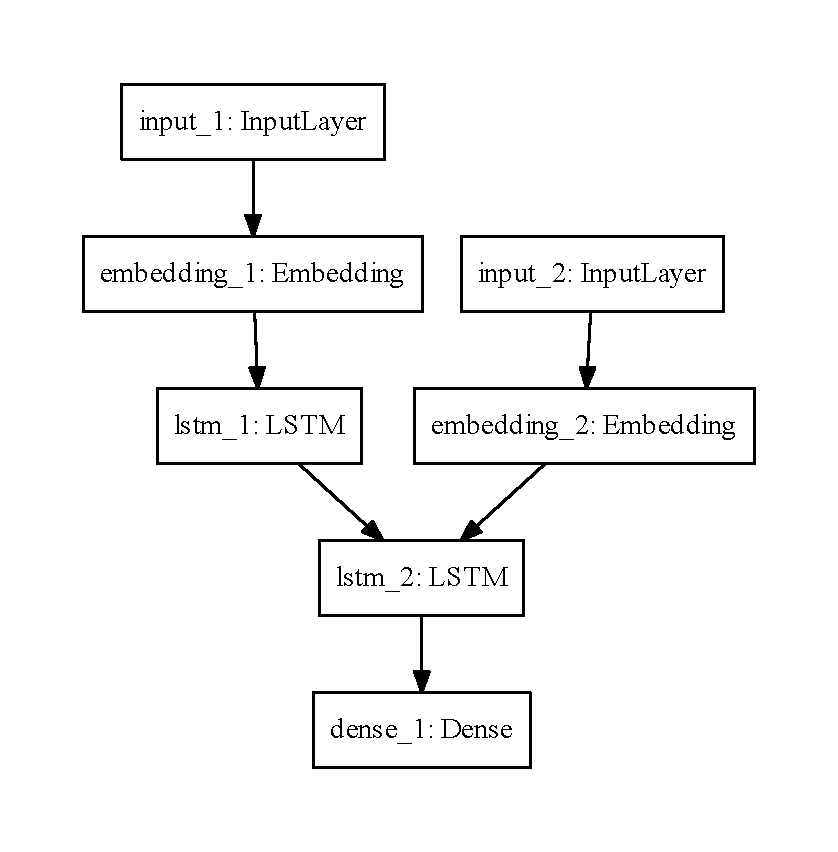
\includegraphics[width=0.95\linewidth]{img/model.pdf}}
    \end{center}
	\caption{Vrstvy a jejich propojení v~enkodér-dekodér modelu použitém při trénovaní za použití jedné vrstvy LSTM pro enkodér a jedné vrstvy LSTM pro dekodér. Do \emph{encoder\_input} přicházejí sekvence ve výchozím jazyce. V~\emph{input\_embeddings} se převedou do podoby embeddings vektoru. Následuje obousměrná vrstva enkodéru. Do \emph{decoder\_input} přichází sekvence začínající startovacím tokenem <s> následovaná korektním překladem v~cílovém jazyce, protože se používá teacher forcing. Do \emph{decoder\_input} přicházejí sekvence v~cílovém jazyce. V~\emph{target\_embeddings} se převedou do podoby embeddings vektoru. Následuje vrstva dekodéru, který je inicializovaný výsledným stavem enkodéru. Zprůměrovaným, protože enkodér je obousměrný, takže má dvojnásobně veliký vnitřní stav. Poslední vrstva \emph{output\_layer} s~aktivační funkcí \emph{softmax} vrací pravděpodobnosti pro všechna slova z~cílového slovníku.}
	\label{img:model}
\end{figure}

\begin{figure}[H]
    \begin{center}
            \tmpframe{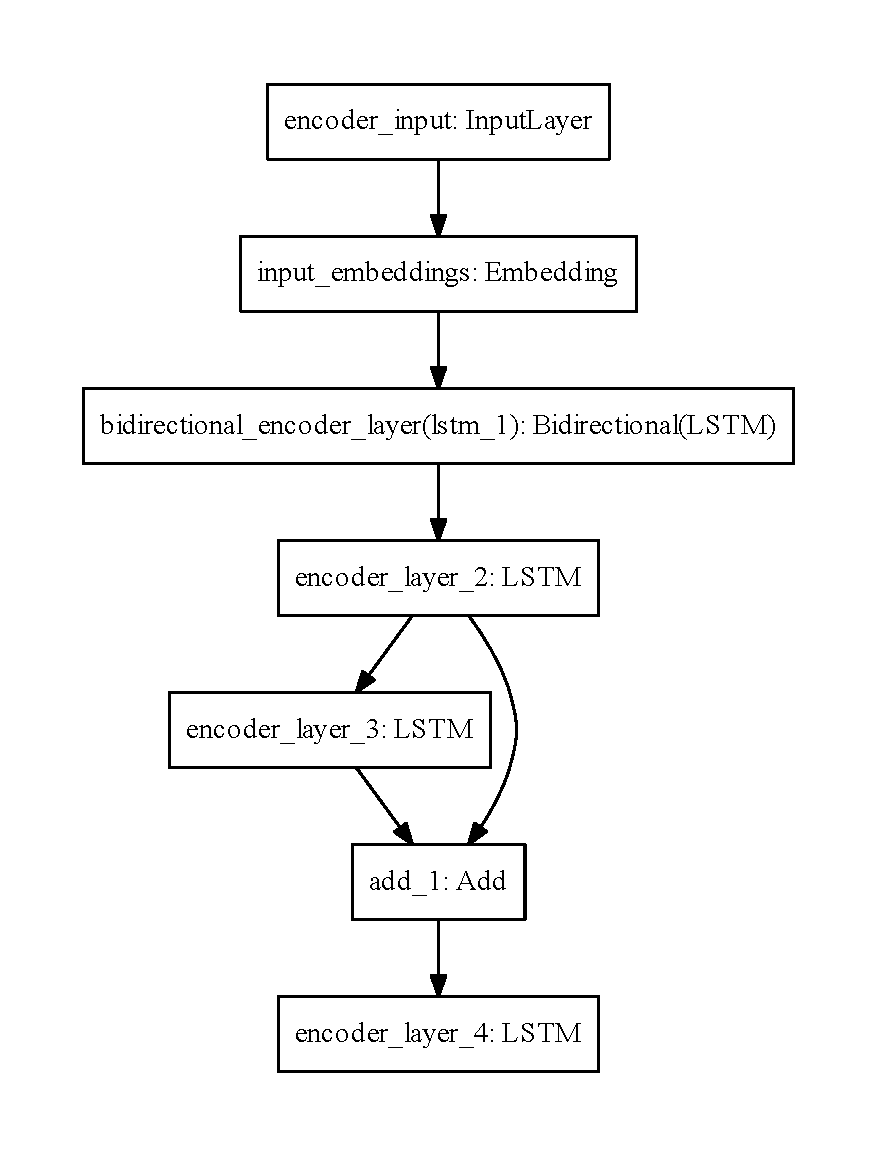
\includegraphics[width=0.6\linewidth]{img/encoder_model.pdf}}
    \end{center}
	\caption{Vrstvy a jejich propojení v~modelu enkodéru použitém při generování překladů při použití tří vrstev LSTM. První vrstva je obousměrná, další vrstvy jsou již jen dopředné. Protože velikost embeddings se nemusí shodovat s~počtem použitých jednotek v~LSTM a první vrstva je obousměrná, reziduální propojení se používá až od třetí vrstvy a dál.}
	\label{img:encodermodel}
\end{figure}

\begin{figure}[H]
    \begin{center}
            \tmpframe{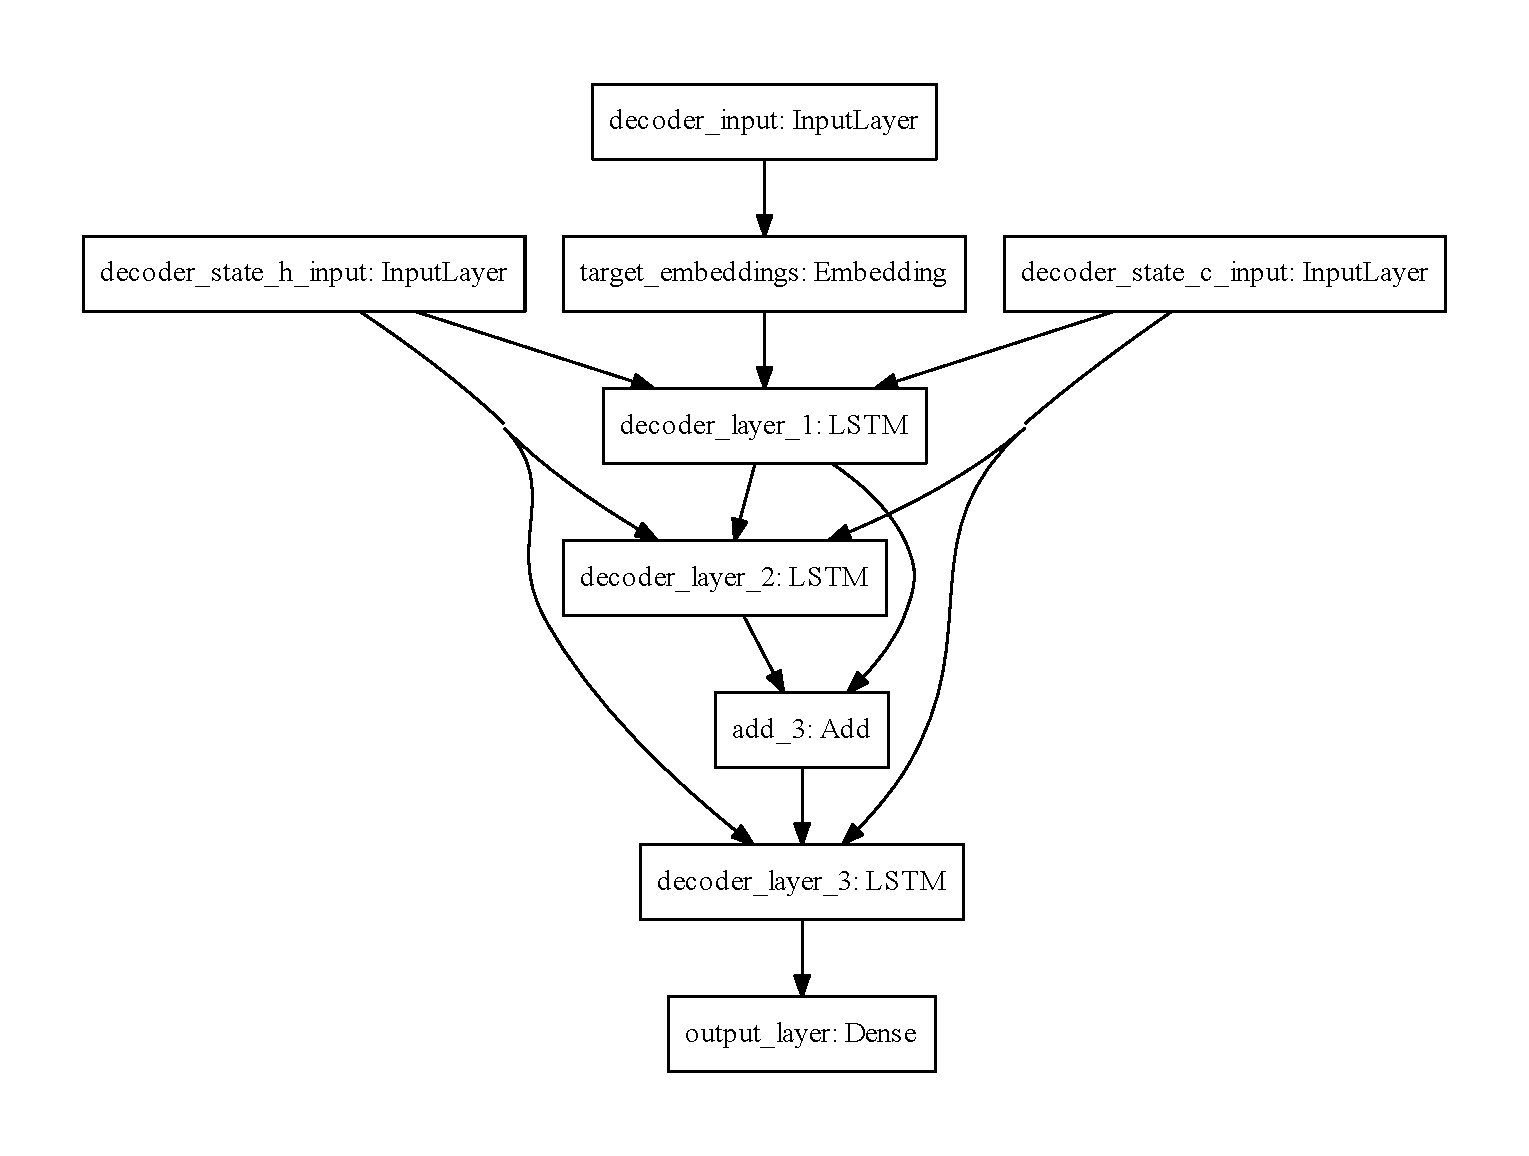
\includegraphics[width=1.0\linewidth]{img/decoder_model.pdf}}
    \end{center}
	\caption{Vrstvy a jejich propojení v~modelu dekodéru použitém při generování překladů při použití 3 vrstev LSTM. Každá vrstva dekodéru je inicializována koncovým stavem enkodéru. Protože velikost embeddings se nemusí shodovat s~počtem použitých jednotek v~LSTM, reziduální propojení se používá až od druhé vrstvy a dál.}
	\label{img:decodermodel}
\end{figure}


%Metodou \emph{fit} se spustí trénování modelu \todo{nekde vysvetlit pojmy jako epocha, batch size a vsechny tyhle dalsi veci..kde a jak?}


\subsubsection{Stručný popis obsahu \texttt{nmt}}
\begin{description}
  \item[třída Translator:] Je hlavní třídou. Přijímá veškerá nastavení týkající se modelu, trénovací a testovací dataset, vytváří model a provádí trénink, překlad a jeho vyhodnocení.

      Přehled hlavních metod:
      \begin{itemize}
                  \item metoda \texttt{fit} zahajuje trénování
                  \item metoda \texttt{translate\_test\_data} přeloží testovací dataset s~pomocí natrénovaného modelu
                  \item metoda \texttt{get\_bleu\_for\_test\_data\_translation} vyhodnotí skóre BLEU pro vzniklý překlad
      \end{itemize}

      Všechny parametry třídy \emph{Translator} jsou popsány v~příloze \ref{append:parameters}.

  \item[třída Dataset:] Drží v~sobě dataset v~jeho tokenizované formě, tedy pole sekvencí jednotlivých vět. Řeší jeho načtení ze souboru a zpracování do podoby vhodné pro trénování.
  \item[třída Vocabulary:] Na základě všech sekvencí v~datasetu daného jazyka vezme a drží v~sobě \emph{n} nejčastějších slov, se kterými pak model pracuje.
  \item[třída Candidate:] Je pomocná třída použitá při výpočtu paprskového prohledávání \ref{decsription:beamsearch}. Drží v~sobě hodnotu jednoho z~aktuálně rozgerovaných kandidátních překladů.
  \item[třída SpecialSymbols:] Obsahuje výčet speciálních symbolů použitých při trénování. \begin{itemize}
                  \item \emph{\_PAD} pro zarovnávací nulu
                  \item \emph{\_GO} pro startovací token
                  \item \emph{\_EOS} pro koncový token
                  \item \emph{\_UNK} pro neznámý token
                \end{itemize}
  \item[třída Utils:] Obsahuje pomocné metody pro úpravu dat, výpočty a pro volání přiložených skriptů jako je \emph{SubwordNMT} a výpočet BLEU skóre.
  \item[knhovna SubwordNMT:] Součástí repozitáře je knihovna \emph{SubwordNMT} použitá pro aplikování BPE (\ref{description:bpeApplication}). Knihovna je přiložena jako \emph{git submodule}.
  \item[testy:] Repozitář \emph{nmt} obsahuje sadu testů pokrývajících jeho funkcionalitu, převážně jednotlivých metod (unit testy) a celkového fungování trénování a překladu. Testy jsou implementovány ve frameworku \emph{pytest}.
\end{description}

\subsection{Rozdělení dat podle velikosti}\label{subsection:Bucketing}
Všechny sekvence při trénování v~rámci jedné dávky musí mít stejnou délku. Věty však mají délku různou. To bývá řešeno tak, že se každá věta zarovná pomocí nul nebo zarovnávacího tokenu na délku nejdelší věty (obrázek \ref{figure:padding}). Na první pohled může být jasné, že pokud se všechny věty v~datasetu zarovnají na velikost nejdelší věty, způsobí to zbytečně větší vytížení paměti a delší trénování modelu.

\begin{figure}[H]
    \begin{center}
        \begin{tabular}{|l|}
          \hline
          \uv{Venku dneska svítí slunce .} \\
          \uv{Ahoj světe .} \\
          \hline
        \end{tabular}
        $\Longrightarrow$
        \begin{tabular}{|l|}
          \hline
          {[1, 2, 3, 4, 5]} \\
          {[6, 7, 5, 0, 0]} \\
          \hline
        \end{tabular}
    \end{center}
	\caption{Příklad zarovnání sekvencí na stejnou délku. V~levé tabulce jsou ukázány věty po tokenizaci, první věta má pět tokenů a druhá tři. V~druhé tabulce jsou pak věty převedené do matic, kde číslo vyjadřuje pozici daného slova ve slovníku respektive v~embeddings a 0 se používá k~zarovnání.}
	\label{figure:padding}
\end{figure}

Tento problém je omezen pomocí rozdělení vět v~datasetech do skupin podle jejich velikostí. Věty o~podobné velikosti jsou shluknuty do jedné skupiny a tím se zamezí zbytečnému nárůstu požadavků na paměť. Dávky se pak při generování (popsáno v~sekci \ref{subsection:generation}) berou vždy z~jedné skupiny tak, aby všechny sekevence v~jedné dávce byly stejně dlouhé.

\subsection{Generování dávek}\label{subsection:generation}
Protože se data při trénování upravují datasety do podoby velkých matic, není možné, kvůli paměťovým omezením, vyrobit jednu matici pro všechna data zaráz. Proto se dávky (batche) v~průběhu trénování vytváří postupně, pomocí generátorové funkce. Ta před každou epochou (jedna epocha znamená, že modelem prošla všechna vstupní data), zamíchá vstupní data. Správné míchání vstupních dat je důležité pro dobrou konvergenci modelu. Dále postupně generuje matice s~jednotlivými dávkami. V~případě, že je použité dělení do skupin podle velikosti, probíhá míchání na úrovni skupin a dávek tak, aby se model nepřetrénoval v~jednu chvíli na například krátké věty a v~jiné části epochy zase na dlouhé. Je použit \texttt{random.seed(0)} pro opakovatelnost experimentů.

\chapter{Experimenty a výsledky} \label{chapter:results}
V~této sekci jsou prezentovány experimenty prováděné na vytvořeném a na referenčním systému. Všechny experimenty byly pouštěny na výpočetním clusteru VUT FIT\footnote{\url{http://www.fit.vutbr.cz/CVT/cluster/}} na GPU.

V~experimentech \ref{subsection:experimentsOptimal} byl systém natrénován pro překlad z~češtiny (cs) do angličtiny (en). Tyto experimenty byly provedeny za účelem najití nejlepších hyperparametrů pro model a pro jeho otestování.

V~experimentu \ref{experimentBestModel} byl systém s nejlepšími parametry vyhodnocen na testovacím datasetu.

V~experimentu \ref{experimentMultiLingual} byl systém natrénován pro překlad mezi více jazyky za pomoci nejlepších parametrů zjištěných z~předchozích experimentů.

Pro všechny experimenty byly použity předučené word embeddings, jak pro vstupní tak výstupní jazyk, poskytnuté firmou Facebook\footnote{\url{https://github.com/facebookresearch/fastText/blob/master/pretrained-vectors.md}}.

Jako optimalizační metoda byl použit RMSprop (\cite{gradientDescent}) s~koeficientem učení 0.001. Každý experiment běžel tak dlouho, dokud se po dobu pěti epoch nezlepšil výsledek loss funkce počítané pro validační dataset. Z~experimentu se ukládají váhy modelu s~nejlepším výsledkem loss funkce.

Použitá velikost jedné trénovací dávky je 128. Je použito generování dávek (\ref{subsection:generation}) a rozdělení dat podle velikosti (\ref{subsection:Bucketing}).

Hodnotící metrikou je standardní skóre BLEU (\ref{subsection:bleu}), protože je to nejčastěji používaná metrika a je použita i ve všech citovaných pracích. Čím větší skóre, tím lepší výsledek. Pro jeho výpočet byl použit skript \emph{multi-blue.pl} dodávaný s~nástrojem Moses.


\section{Použité datasety}
Všechny použité datasety pocházejí z~každoročně publikovaného překládacího úkolu konference o~strojovém překladu \textbf{WMT} (dříve \textbf{w}orkshop on statistical \textbf{m}achine \textbf{t}ranslation). Konkrétně jsou použity datasety z~WMT17\footnote{\url{http://data.statmt.org/wmt17/translation-task/preprocessed/}} obsahující textová data z~různých domén, jako jsou titulky, knihy, noviny a internet.

Stažené datasety byly rozdělený na několik menších datasetů, které spolu nesdílí páry vět. Následuje jejich popis a přehled v tabulce \ref{table:datasets}.
\begin{description}
  \item[$Cs\rightarrow En$ trénovací dataset:] Obsahuje milion párů vět. Je určený pro trénování v~experimentech, pomocí kterých se hledají optimální hyperparametry modelu a pro trénování referenčního systému.
  \item[$Cs\rightarrow En$ validační dataset:] Obsahuje dva tisíce párů vět. Je určený pro testování modelu trénovaném s~malým trénovacím datasetem za účelem hledání optimálních hyperparametrů modelu.
  \item[$Cs\rightarrow En$ testovací dataset:] Obsahuje dva tisíce párů vět. Je určený pro finální otestování modelu natrénovaného s nejlepšími nalezenými parametry. Používá se místo validačního modelu aby se vyzkoušelo, že výsledný model je skutečně schopný generalizace a nebyl jen úzce přizpůsoben pro dobré výsledky s~validačním datasetem.
  \item[$En\rightarrow De$ trénovací dataset:] Obsahuje milion párů vět. Je určený pro trénování modelu pro překlad nad více jazyky.
  \item[$En\rightarrow De$ testovací dataset:] Obsahuje dva tisíce párů vět. Je určený pro otestování překladu nad více jazyky.
  \item[$Cs\rightarrow De$ testovací dataset:] Obsahuje dva tisíce párů vět. Je určený pro otestování zero-shot překladu, tedy překladu, pro který model nebyl explicitně natrénován.
\end{description}

\begin{table}[H]
    \begin{center}
        \begin{tabular}{ll}
          \toprule
          dataset & počet párů vět  \\
          \midrule
          $Cs\rightarrow En$ trénovací & 1 000 000 \\
          $Cs\rightarrow En$ validační & 2 000 \\
          $Cs\rightarrow En$ testovací & 2 000 \\
          $En\rightarrow De$ trénovací & 1 000 000 \\
          $En\rightarrow De$ testovací & 2 000 \\
          $Cs\rightarrow De$ testovací & 2 000 \\
          \bottomrule
        \end{tabular}
    \end{center}
	\caption{Přehled použitých datasetů a pro každý z nich, kolik obsahuje párů vět.}
	\label{table:datasets}
\end{table}

V~případě, že byl dataset v~experimentu předzpracován pomocí subword-nmt pro rozdělení slov na menší jednotky, byl vždy přeložený text před vyhodnocením BLEU skóre převeden zpátky na celá slova.

\section{Referenční systém v~Moses}
Systém (popsaný v~\ref{section:referent}) byl natrénován za účelem porovnání jeho výsledku s~výsledky prezentovaného systému. Pro trénování byl použit $Cs\rightarrow En$ \textbf{trénovací dataset} a pro vyhodnocení $Cs\rightarrow En$ \textbf{testovací dataset}. Výsledek je v~tabulce \ref{table:referent}.

\begin{table}[H]
    \begin{center}
        \begin{tabular}{ll}
          \toprule
          model & BLEU skóre  \\
          \midrule
          referenční z nástroje Moses & 23.08\\
          \bottomrule
        \end{tabular}
    \end{center}
	\caption{Výsledky modelu natrénovaného pomocí statistického nástroje Moses v4.0.}
	\label{table:referent}
\end{table}

\section{Experimenty}

\subsection{Hledání optimálních hyperparametrů}\label{subsection:experimentsOptimal}
V~této sekci je popsán průběh a výsledky experimentů prováděných za účelem nalezení co nejlepších hyperparametrů modelu. Všechny experimenty jsou provedeny na překladu z~češtiny do angličtiny za pomocí $Cs\rightarrow En$ \textbf{trénovacího datasetu} a překlad je testován pomocí $Cs\rightarrow En$ \textbf{validačního datasetu}.

\subsubsection{1. experiment -- baseline -- WordsEn1-512Dec1-512Voc15000Beam1}\label{experiment1}
Model a jeho parametry z~tohoto experimentu bude považován za baseline vůči kterému budou porovnány výsledky modelů z~dalších experimentů, aby se dalo určit, k~jak velkému došlo vylepšení.

Parametry:
\begin{itemize}
  \item používají se celá slova
  \item jedna vrstva LSTM v~enkodéru o~velikosti 512
  \item jedna vrstva LSTM v~dekodéru o~velikosti 512
  \item velikost slovníku je omezena na 15000
  \item paprskové prohledávání o~velikosti 1
\end{itemize}

Trénování bylo ukončeno po 9. epoše. Nejlepší dosažený výsledek \textbf{loss funkce} pro validační dataset je \textbf{2.855}. \textbf{Skóre BLEU} překladu vygenerovaného pro validační dataset je \textbf{7.26}. Pro možnost porovnání s~výsledným nejlepším modelem byl proveden překlad i testovacího datasetu a to se \textbf{skóre 7.36}.

\begin{figure}[H]
    \begin{center}
            \begin{tikzpicture}
            \begin{axis}[grid=both,
                         width=0.45\linewidth,
                         xlabel=epocha,
                         ylabel=loss,
                         xtick=data,
                         legend entries = {trénovací dataset, validační dataset}]
                \addplot table [x=Step, y=Value, col sep=comma] {img/experiments/run_G_final1_logs-tag-loss.csv};
                \addplot table [x=Step, y=Value, col sep=comma] {img/experiments/run_G_final1_logs-tag-val_loss.csv};
            \end{axis}
            \end{tikzpicture}
    \end{center}
	\caption{Průběh vývoje hodnot loss funkce po jednotlivých epochách pro trénovací a validační dataset.}
\end{figure}

\subsubsection{2. experiment -- WordsEn1-512Dec1-512Voc30000Beam1}\label{experiment2}
Parametry:
\begin{itemize}
  \item používají se celá slova
  \item jedna vrstva LSTM v~enkodéru o~velikosti 512
  \item jedna vrstva LSTM v~dekodéru o~velikosti 512
  \item velikost slovníku je omezena na 30000
  \item paprskové prohledávání o~velikosti 1
\end{itemize}

Trénování bylo ukončeno po 11. epoše. Nejlepší dosažený výsledek \textbf{loss funkce} pro validační dataset je \textbf{2.965}. \textbf{Skóre BLEU} překladu vygenerovaného pro validační dataset je \textbf{7.79}. To znamená, že zvětšení maximální velikosti slovníku za cenu značného navýšení velikosti modelu a času trénování přineslo o~něco lepší výsledek.

\begin{figure}[H]
    \begin{center}
            \begin{tikzpicture}
            \begin{axis}[grid=both,
                         width=0.45\linewidth,
                         xlabel=epocha,
                         ylabel=loss,
                         xtick=data,
                         legend entries = {trénovací dataset, validační dataset}]
                \addplot table [x=Step, y=Value, col sep=comma] {img/experiments/run_G_final2_logs-tag-loss.csv};
                \addplot table [x=Step, y=Value, col sep=comma] {img/experiments/run_G_final2_logs-tag-val_loss.csv};
            \end{axis}
            \end{tikzpicture}
    \end{center}
	\caption{Průběh vývoje hodnot loss funkce po jednotlivých epochách pro trénovací a validační dataset.}
\end{figure}


\subsubsection{3. experiment -- SubwordsEn1-512Dec1-512Voc15000Beam1}\label{experiment3}
Parametry:
\begin{itemize}
  \item slova jsou rozdělena na menší jednotky
  \item jedna vrstva LSTM v~enkodéru o~velikosti 512
  \item jedna vrstva LSTM v~dekodéru o~velikosti 512
  \item velikost slovníku je omezena na 15000
  \item paprskové prohledávání o~velikosti 1
\end{itemize}

Trénování bylo ukončeno po 11. epoše. Nejlepší dosažený výsledek \textbf{loss funkce} pro validační dataset je \textbf{3.090}. \textbf{Skóre BLEU} překladu vygenerovaného pro validační dataset je \textbf{8.37}. Při zachování parametrů z~experimentu \ref{experiment1} a použití BPE je výsledné skóre lepší a to bez zvětšení velikosti modelu a navýšení doby trénování. Všechny další experimenty budou proto prováděny s~použitím BPE a subword units.

\begin{figure}[H]
    \begin{center}
            \begin{tikzpicture}
            \begin{axis}[grid=both,
                         width=0.45\linewidth,
                         xlabel=epocha,
                         ylabel=loss,
                         xtick=data,
                         legend entries = {trénovací dataset, validační dataset}]
                \addplot table [x=Step, y=Value, col sep=comma] {img/experiments/run_G_final3_logs-tag-loss.csv};
                \addplot table [x=Step, y=Value, col sep=comma] {img/experiments/run_G_final3_logs-tag-val_loss.csv};
            \end{axis}
            \end{tikzpicture}
    \end{center}
	\caption{Průběh vývoje hodnot loss funkce po jednotlivých epochách pro trénovací a validační dataset.}
\end{figure}

\subsubsection{4. experiment -- SubwordsEn1-1000Dec1-1000Voc15000Beam1-15}\label{experiment4}
Parametry:
\begin{itemize}
  \item slova jsou rozdělena na menší jednotky
  \item jedna vrstva LSTM v~enkodéru o~velikosti 1000
  \item jedna vrstva LSTM v~dekodéru o~velikosti 1000
  \item velikost slovníku je omezena na 15000
  \item paprskové prohledávání o~velikosti 1, 5, 8, 10, 12, 15
\end{itemize}

Trénování bylo ukončeno po 10. epoše. Nejlepší dosažený výsledek \textbf{loss funkce} pro validační dataset je \textbf{3.016}. Kromě zvýšení velikosti jednotek LSTM byl také testován vliv použité velikosti paprskového prohledávání při generování překladů. Výsledky jsou v~tabulce \ref{table:resultsExperiment4} a ukázka zlepšení překladů je v~tabulce \ref{table:beamTranslation}. Jak navýšení počtu jednotek, tak velikost paprskového prohledávání přineslo lepší výsledek a bude tak používáno v~dalších experimentech.

\begin{figure}[H]
    \begin{center}
            \begin{tikzpicture}
            \begin{axis}[grid=both,
                         width=0.45\linewidth,
                         xlabel=epocha,
                         ylabel=loss,
                         xtick=data,
                         legend entries = {trénovací dataset, validační dataset}]
                \addplot table [x=Step, y=Value, col sep=comma] {img/experiments/run_G_final4_logs-tag-loss.csv};
                \addplot table [x=Step, y=Value, col sep=comma] {img/experiments/run_G_final4_logs-tag-val_loss.csv};
            \end{axis}
            \end{tikzpicture}
    \end{center}
	\caption{Průběh vývoje hodnot loss funkce po jednotlivých epochách pro trénovací a validační dataset.}
\end{figure}

\begin{table}[H]
    \begin{center}
        \begin{tabular}{ll}
          \toprule
          velikost paprskové prohledávání & BLEU skóre \\
          \midrule
          1 & 8.75 \\
          5 & 9.34 \\
          8 & 9.4 \\
          10 & 9.41 \\
          12 & 9.43 \\
          \textbf{15} & \textbf{9.47} \\
          \bottomrule
        \end{tabular}
    \end{center}
	\caption{Porovnání výsledků pro různou velikost paprskového prohledávání. Nejlepší výsledek byl dosažen z velikostí 15.}
	\label{table:resultsExperiment4}
\end{table}

\begin{table}[H]
    \begin{center}
        \begin{tabular}{ll}
          \toprule
          původní věta v~češtině & žádní pánové už nejsou. \\
          překlad při velikosti 1 & no more gentlemen. \\
          překlad při velikosti 5 & there are no more men. \\
          překlad při velikosti 15 & there are no gentlemen no more. \\
          \bottomrule
        \end{tabular}
    \end{center}
	\caption{Ukázka zlepšení překladu při použití různých velikostí paprskového prohledávání.}
	\label{table:beamTranslation}
\end{table}

\subsubsection{5. experiment -- SubwordsEn1-1000Dec1-1000Voc15000Beam15Dropout0.1-0.3}\label{experiment5}
Parametry:
\begin{itemize}
  \item slova jsou rozdělena na menší jednotky
  \item jedna vrstva LSTM v~enkodéru o~velikosti 1000
  \item jedna vrstva LSTM v~dekodéru o~velikosti 1000
  \item velikost slovníku je omezena na 15000
  \item paprskové prohledávání o~velikosti 15
  \item dropout o~velikosti 0.1, 0.2, 0.3
\end{itemize}

 Pro dropout 0.1 bylo trénování ukončeno po 10. epoše. Pro hodnoty 0.2 a 0.3 po 13. epoše, protože model se může déle trénovat bez přetrénování. Nejlepší dosažený výsledek \textbf{loss funkce} pro validační dataset je \textbf{2.944}. Výsledky jsou v~tabulce \ref{table:resultsExperiment5}. Nejlepšího skóre bylo dosaženo pro dropout 0.1, takže tato hodnota bude použita v~dalších experimentech.

\begin{figure}[H]
    \begin{center}
            \begin{tikzpicture}
            \begin{axis}[grid=both,
                         width=0.48\linewidth,
                         xlabel=epocha,
                         ylabel=loss,
                         minor xtick={1,3,...,13},
                         xtick={0,2, ..., 12},
                         legend entries = {dropout=0.1, dropout=0.2, dropout=0.3}]
                \addplot table [x=Step, y=Value, col sep=comma] {img/experiments/run_G_final5-2_logs-tag-loss.csv};
                \addplot table [x=Step, y=Value, col sep=comma] {img/experiments/run_G_final5_logs-tag-loss.csv};
                \addplot table [x=Step, y=Value, col sep=comma] {img/experiments/run_G_final5-3_logs-tag-loss.csv};
            \end{axis}
            \end{tikzpicture}
            \begin{tikzpicture}
            \begin{axis}[grid=both,
                         width=0.48\linewidth,
                         xlabel=epocha,
                         ylabel=val\_loss,
                         minor xtick={1,3,...,13},
                         xtick={0,2, ..., 12},
                         legend entries = {dropout=0.1, dropout=0.2, dropout=0.3}]
                \addplot table [x=Step, y=Value, col sep=comma] {img/experiments/run_G_final5-2_logs-tag-val_loss.csv};
                \addplot table [x=Step, y=Value, col sep=comma] {img/experiments/run_G_final5_logs-tag-val_loss.csv};
                \addplot table [x=Step, y=Value, col sep=comma] {img/experiments/run_G_final5-3_logs-tag-val_loss.csv};
            \end{axis}
            \end{tikzpicture}
    \end{center}
	\caption{Průběh vývoje hodnot loss funkce po jednotlivých epochách. Levý graf je pro trénovací dataset a pravý pro validační dataset.}
\end{figure}

\begin{table}[H]
    \begin{center}
        \begin{tabular}{ll}
          \toprule
          velikost dropout & BLEU skóre \\
          \midrule
           0.1 & 10.02 \\
           0.2 &  9.39 \\
           0.3 &  9.62 \\
          \bottomrule
        \end{tabular}
    \end{center}
	\caption{Porovnání výsledků při použití různé hodnoty dropout.}
	\label{table:resultsExperiment5}
\end{table}

\subsubsection{6. experiment -- SubwordsEn2-1000Dec1-1000Voc15000Beam15Dropout0.1}\label{experiment6}
Parametry:
\begin{itemize}
  \item slova jsou rozdělena na menší jednotky
  \item dvě vrstvy LSTM v~enkodéru o~velikosti 1000
  \item jedna vrstva LSTM v~dekodéru o~velikosti 1000
  \item velikost slovníku je omezena na 15000
  \item paprskové prohledávání o~velikosti 15
  \item dropout 0.1
\end{itemize}

Trénování bylo ukončeno po 13. epoše. Nejlepší dosažený výsledek \textbf{loss funkce} pro validační dataset je \textbf{2.930}. \textbf{Skóre BLEU} překladu vygenerovaného pro validační dataset je \textbf{9.99}.

\begin{figure}[H]
    \begin{center}
            \begin{tikzpicture}
            \begin{axis}[grid=both,
                         width=0.45\linewidth,
                         xlabel=epocha,
                         ylabel=loss,
                         xtick=data,
                         legend entries = {trénovací dataset, validační dataset}]
                \addplot table [x=Step, y=Value, col sep=comma] {img/experiments/run_G_final6_logs-tag-loss.csv};
                \addplot table [x=Step, y=Value, col sep=comma] {img/experiments/run_G_final6_logs-tag-val_loss.csv};
            \end{axis}
            \end{tikzpicture}
    \end{center}
	\caption{Průběh vývoje hodnot loss funkce po jednotlivých epochách pro trénovací a validační dataset.}
\end{figure}

\subsubsection{7. experiment -- SubwordsEn1-1000Dec2-1000Voc15000Beam15Dropout0.1}\label{experiment7}
Parametry:
\begin{itemize}
  \item slova jsou rozdělena na menší jednotky
  \item jedna vrstva LSTM v~enkodéru o~velikosti 1000
  \item dvě vrstvy LSTM v~dekodéru o~velikosti 1000
  \item velikost slovníku je omezena na 15000
  \item paprskové prohledávání o~velikosti 15
  \item dropout 0.1
\end{itemize}

Trénování bylo ukončeno po 12. epoše. Nejlepší dosažený výsledek \textbf{loss funkce} pro validační dataset je \textbf{2.835}. \textbf{Skóre BLEU} překladu vygenerovaného pro validační dataset je \textbf{10.14}.

\begin{figure}[H]
    \begin{center}
            \begin{tikzpicture}
            \begin{axis}[grid=both,
                         width=0.45\linewidth,
                         xlabel=epocha,
                         ylabel=loss,
                         xtick=data,
                         legend entries = {trénovací dataset, validační dataset}]
                \addplot table [x=Step, y=Value, col sep=comma] {img/experiments/run_G_final7_logs-tag-loss.csv};
                \addplot table [x=Step, y=Value, col sep=comma] {img/experiments/run_G_final7_logs-tag-val_loss.csv};
            \end{axis}
            \end{tikzpicture}
    \end{center}
	\caption{Průběh vývoje hodnot loss funkce po jednotlivých epochách pro trénovací a validační dataset.}
\end{figure}


\subsubsection{8. experiment -- SubwordsEn2-1000Dec2-1000Voc15000Beam15Dropout0.1}\label{experiment8}
Parametry:
\begin{itemize}
  \item slova jsou rozdělena na menší jednotky
  \item dvě vrstvy LSTM v~enkodéru o~velikosti 1000
  \item dvě vrstvy LSTM v~dekodéru o~velikosti 1000
  \item velikost slovníku je omezena na 15000
  \item paprskové prohledávání o~velikosti 15
  \item dropout 0.1
\end{itemize}

Trénování bylo ukončeno po 13. epoše. Nejlepší dosažený výsledek \textbf{loss funkce} pro validační dataset je \textbf{2.817}. \textbf{Skóre BLEU} překladu vygenerovaného pro validační dataset je \textbf{10.42}.

\begin{figure}[H]
    \begin{center}
            \begin{tikzpicture}
            \begin{axis}[grid=both,
                         width=0.45\linewidth,
                         xlabel=epocha,
                         ylabel=loss,
                         xtick=data,
                         legend entries = {trénovací dataset, validační dataset}]
                \addplot table [x=Step, y=Value, col sep=comma] {img/experiments/run_G_final8_logs-tag-loss.csv};
                \addplot table [x=Step, y=Value, col sep=comma] {img/experiments/run_G_final8_logs-tag-val_loss.csv};
            \end{axis}
            \end{tikzpicture}
    \end{center}
	\caption{Průběh vývoje hodnot loss funkce po jednotlivých epochách pro trénovací a validační dataset.}
\end{figure}

\subsubsection{9. experiment -- SubwordsEn4-1000Dec4-1000Voc15000Beam15Dropout0.1}\label{experiment9}
Parametry:
\begin{itemize}
  \item slova jsou rozdělena na menší jednotky
  \item čtyři vrstvy LSTM v~enkodéru o~velikosti 1000
  \item čtyři vrstvy LSTM v~dekodéru o~velikosti 1000
  \item velikost slovníku je omezena na 15000
  \item paprskové prohledávání o~velikosti 15
  \item dropout 0.1
\end{itemize}

Trénování bylo ukončeno po 12. epoše. Nejlepší dosažený výsledek \textbf{loss funkce} pro validační dataset je \textbf{2.818}. \textbf{Skóre BLEU} překladu vygenerovaného pro validační dataset je \textbf{9.78}, takže nejlepším modelem zůstavá model z~experimentu \ref{experiment8}.

\begin{figure}[H]
    \begin{center}
            \begin{tikzpicture}
            \begin{axis}[grid=both,
                         width=0.45\linewidth,
                         xlabel=epocha,
                         ylabel=loss,
                         xtick=data,
                         legend entries = {trénovací dataset, validační dataset}]
                \addplot table [x=Step, y=Value, col sep=comma] {img/experiments/run_G_final9_logs-tag-loss.csv};
                \addplot table [x=Step, y=Value, col sep=comma] {img/experiments/run_G_final9_logs-tag-val_loss.csv};
            \end{axis}
            \end{tikzpicture}
    \end{center}
	\caption{Průběh vývoje hodnot loss funkce po jednotlivých epochách pro trénovací a validační dataset.}
\end{figure}

\subsubsection{Shrnutí}\label{experimentsSummary}
V tabulce \ref{table:experimentSummary} je shrnutí výsledků všech experimentů provedených za účelem nalezení nejlepších hyperparametrů.

\begin{table}[H]
    \begin{center}
        \begin{tabular}{ll}
          \toprule
          model & BLEU skóre\\
          \midrule
          Baseline -- WordsEn1-512Dec1-512Voc15000Beam1 & 7.36 \\
          WordsEn1-512Dec1-512Voc30000Beam1 & 7.79 \\
          SubwordsEn1-512Dec1-512Voc15000Beam1 & 8.37 \\
          SubwordsEn1-1000Dec1-1000Voc15000Beam15 & 9.47 \\
          SubwordsEn1-1000Dec1-1000Voc15000Beam15Dropout0.1 & 10.02 \\
          SubwordsEn2-1000Dec1-1000Voc15000Beam15Dropout0.1 & 9.99 \\
          SubwordsEn1-1000Dec2-1000Voc15000Beam15Dropout0.1 & 10.14 \\
          SubwordsEn2-1000Dec2-1000Voc15000Beam15Dropout0.1 & \textbf{10.42} \\
           SubwordsEn4-1000Dec4-1000Voc15000Beam15Dropout0.1 & 9.78 \\
          \bottomrule
        \end{tabular}
    \end{center}
	\caption{Výsledky všech experimentů prováděných na $Cs\rightarrow En$ datasetu za účelem nalezení nejlepších hyperparametrů.}
	\label{table:experimentSummary}
\end{table}


\subsection{Otestování nejlepšího modelu} \label{experimentBestModel}
Modelem s~nejlepšími dosaženými výsledky je model s~parametry z~experimentu \ref{experiment8}. Výsledky jeho překladu pro testovací dataset jsou v~tabulce \ref{table:bestResults}.

\begin{table}[H]
    \begin{center}
        \begin{tabular}{ll}
          \toprule
          model & BLEU skóre \\
          \midrule
          SubwordsEn2-1000Dec2-1000Voc15000Beam15Dropout0.1 & 9.87 \\
          \bottomrule
        \end{tabular}
    \end{center}
	\caption{Výsledné skóre BLEU nad $Cs\rightarrow En$ testovacím datasetem. Překlad byl proveden s~modelem, který dosáhl nejlepších výsledků pro validační dataset.}
	\label{table:bestResults}
\end{table}


\subsection{Překlad mezi více jazyky} \label{experimentMultiLingual}
V~této sekci je popsán experiment, kdy se jeden model trénuje na překlad vícero jazykových párů. Trénovací dataset vznikl spojením a promícháním trénovacího $Cs\rightarrow En$ datasetu a trénovacího $En\rightarrow De$ datasetu. Před věty ve výchozím jazyce se přidal token jazyku do kterého se překládají, tak jak je uvedeno v~sekci \ref{section:multilingual}. Model natrénovaný na těchto datech by tedy měl umět překládat z~češtiny do angličtiny, z~angličtiny do němčiny a možná trochu z~češtiny do němčiny.

Použité parametry jsou stejné jako v~experimentu \ref{experiment8}, tedy parametry se kterými model dosáhl nejlepších výsledků. Trénování bylo ukončeno po 7. epoše. Nejlepší dosažený výsledek \textbf{loss funkce} pro validační dataset je \textbf{3.447}. \textbf{Skóre BLEU} pro všechny testované jazykové páry jsou v~tabulce \ref{table:resultsMulti}.

\begin{figure}[H]
    \begin{center}
            \begin{tikzpicture}
            \begin{axis}[grid=both,
                         width=0.45\linewidth,
                         xlabel=epocha,
                         ylabel=loss,
                         xtick=data,
                         legend entries = {trénovací dataset, validační dataset},
                         legend pos=outer north east]
                \addplot table [x=Step, y=Value, col sep=comma] {img/experiments/run_G_final11_logs-tag-loss.csv};
                \addplot table [x=Step, y=Value, col sep=comma] {img/experiments/run_G_final11_logs-tag-val_loss.csv};
            \end{axis}
            \end{tikzpicture}
    \end{center}
	\caption{Průběh vývoje hodnot loss funkce po jednotlivých epochách pro trénovací a validační dataset.}
\end{figure}

\begin{table}[H]
    \begin{center}
        \begin{tabular}{ll}
          \toprule
          jazykový pár & skóre BLEU \\
          \midrule
          $Cs\rightarrow En$ & 7.10 \\
          $En\rightarrow De$ & 7.39 \\
          $Cs\rightarrow De$ &  0.14 \\
          \bottomrule
        \end{tabular}
    \end{center}
	\caption{Výsledné skóre BLEU pro testovací datasety různých jazykových párů. Překlad byl proveden jedním modelem natrénovaným na párech $Cs\rightarrow En$ a $En\rightarrow De$. Výsledky ukazují, že model je schopný překládat pro oba natrénované páry, ale za cenu horšího výsledku pro $Cs\rightarrow En$, než když byl natrénován jen pro tento jeden pár. Zero-shot překlad páru $Cs\rightarrow De$ nevykazuje úspěch.}
	\label{table:resultsMulti}
\end{table}

\subsection{Výsledky}
Všechny dosažené výsledky jsou shrnuty v~tabulce \ref{table:results}. Ukázky překladů pro $Cs\rightarrow En$ pár jsou v~tabulce \ref{img:exampleResults}. Doposud se nepodařilo objasnit proč vytvořený model nedosahuje lepších výsledků, a bylo by vhodné to dále v~budoucnu zkoumat.

\begin{table}[H]
    \begin{center}
        \begin{tabular}{lll}
          \toprule
           model & jazykový pár & skóre BLEU \\
          \midrule
           referenční z nástroje Moses & $Cs\rightarrow En$ & 23.08 \\
           baseline model & $Cs\rightarrow En$ & 7.36 \\
           nejúspěšnější vytvořený model & $Cs\rightarrow En$ & 9.87 \\
           více jazykový model & $Cs\rightarrow En$ & 7.10 \\
           více jazykový model & $En\rightarrow De$ & 7.39 \\
           více jazykový model & $Cs\rightarrow De$ & 0.14 \\
          \bottomrule
        \end{tabular}
    \end{center}
	\caption{Dosažené skóre BLEU pro různé modely a jazykové páry. Žádný z~vytvořených modelů pro pár $Cs\rightarrow En$ nedosáhl výsledků referenčního modelu vytvořeného v~nástroji Moses. Nejúspěšnější model z~experimentu \ref{experiment8} dosáhl zlepšení vůči baseline modelu, což se projevuje i na ukázkách překladu \ref{img:exampleResults}. Model natrénovaný pro překlad mezi více jazyky má skóre horší jak baseline model pro překlad $Cs\rightarrow En$, ale za to dosahuje podobného výsledku i pro překlad $Cs\rightarrow De$.}
	\label{table:results}
\end{table}


\begin{table}[H]
    \begin{center}
        \begin{tabular}{p{0.44\linewidth}}
          \toprule
          \multicolumn{1}{c}{originální text} \\
          \midrule
          1. budoucnost se jevila černě. \\
          2. někdo mu musí dát lekci. \\
          3. nejdůležitější výsledky studie jsou uvedeny v~tabulce 4 a na obrázku 3. \\
          4. uvidíme, jak se ta schůze bude odvíjet. \\
          5. Evropská unie je druhým největším obchodním partnerem ASEAN. \\
          6. 13. prosinec \\
          \bottomrule
        \end{tabular}
        \hspace{5mm}
        \begin{tabular}{p{0.44\linewidth}}
          \toprule
          \multicolumn{1}{c}{originální překlad} \\
          \midrule
          1. the future was grey. \\
          2. somebody's~got to teach him a lesson. \\
          3. the key results of the trial are listed in Table 4 and Figure 3. \\
          4. see how the meeting goes. \\
          5. the European Union is ASEAN's~second largest trading partner. \\
          6. December 13 \\
          \bottomrule
        \end{tabular}
    \end{center}
    \begin{center}
        \begin{tabular}{p{0.44\linewidth}}
          \toprule
          \multicolumn{1}{c}{překlad referenčního systému Moses} \\
          \midrule
          1. the jevila black.  \\
          2. someone must give him a lesson.  \\
          3. the study results are provided in Table 4 and the picture 3. \\
          4. we'll see how the meeting is odvíjet. \\
          5. the European Union's~second largest partner ASEAN. \\
          6. 13 December \\
          \bottomrule
        \end{tabular}
        \hspace{5mm}
        \begin{tabular}{p{0.44\linewidth}}
          \toprule
          \multicolumn{1}{c}{překlad baseline modelu} \\
          \midrule
          1. the future future became \_UNK. \\
          2. somebody must teach him a lesson. \\
          3. the following involved interested in the results of the information and the \_UNK are available in the.\\
          4. see how the \_UNK will be happening. \\
          5. the European Union is the European Union \_UNK. \\
          6. 13 \_UNK \\
          \bottomrule
        \end{tabular}
    \end{center}
    \begin{center}
        \begin{tabular}{p{0.44\linewidth}}
          \toprule
          \multicolumn{1}{c}{překlad nejlepšího modelu} \\
          \midrule
          1. the future was red. \\
          2. someone needs to give him a lesson. \\
          3. the most important results of the two and two are available in the level of the 3. \\
          4. let's~see how the meeting goes. \\
          5. the European Agreement is the most attractive partner of the European Union. \\
          6. 13. \\
          \bottomrule
        \end{tabular}
        \hspace{3mm}
        \begin{tabular}{p{0.44\linewidth}}
          \toprule
          \multicolumn{1}{c}{překlad více jazykového modelu} \\
          \midrule
          1. the whole body was ty. \\
          2. someone's~got to take care of him. \\
          3. the same \\
          4. we'll see how it's~going to be done. \\
          5. the the EU's~the right of the ASEE. \\
          6. 13 . ( 1 ) \\
          \bottomrule
        \end{tabular}
    \end{center}
	\caption{Ukázky překladu vět z~testovacího datasetu. V~první tabulce jsou originální věty v~českém jazyce, v~druhé tabulce jsou originální anglické překlady. Ve třetí tabulce je překlad, který vytvořil referenční systém vytvořený v~nástroji Moses, ve čtvrté překlady baseline modelu, v~páté tabulce jsou překlady vytvořené nejlepším dosaženým modelem a v~poslední tabulce jsou překlady modelu trénovaného nad více jazyky. Je vidět že překlad z~Moses si pomáhá přenášením neznámých slov do přeložené věty, což v~případě například jmen může pomoci, ale v~jiných případech jako je první věta může být ke škodě. I~přes nevelkou změnu v~BLEU skóre je vidět značné zlepšení mezi větami přeloženými baseline modelem a modelem s~nejlepším skóre.}
	\label{img:exampleResults}
\end{table}

\chapter{Závěr}
Cílem této práce bylo prozkoumat a vytvořit systém pro strojový překlad s~použitím neuronových sítí. Systém byl vytvořen s~pomocí architektury enkodér-dekodér, která používá jednotek LSTM pro překlad celých vět mezi dvěmi jazyky. Výsledkem je balíček pro Python \emph{nmt}, který je publikován na serveru github na adrese \url{github.com/jojkos/neural-machine-translation} pro veřejné použití.

Pro trénink a otestování modelu vytvořeného vytvořeným systémem byla zvolena data z~konference WMT. Byla provedena řada experimentů pro získání hyperparametrů, se kterými model dosahuje nejlepších výsledků. Experimenty byly prováděny nad jazykovým párem $Cs\rightarrow En$ pro který měl trénovací dataset 1 milion párů vět. Výsledky jsou hodnoceny pomocí standardní metriky BLEU kde vyšší skóre znamená lepší výsledek. Model s~nejlepším výkonem dosáhl při překladu $Cs\rightarrow En$ skóre \textbf{9.87}. Pro porovnání byl na stejných trénovacích datech natrénován systém vytvořený nástrojem Moses, který pro stejná testovací data dosáhl skóre \textbf{23.08}, tedy lepšího výsledku.

Dále byl proveden experiment, ve kterém byl model natrénován pro překlad mezi více jazykovými páry, konkrétně $Cs\rightarrow En$ a $En\rightarrow De$. Pro každý jazykový pár obsahoval trénovací dataset 1 milion párů vět. Tento model dosáhl výsledků \textbf{7.10} pro první jazykový pár a \textbf{7.39} pro druhý. Za cenu mírného zhoršení překladu pro $Cs\rightarrow En$ je jeden model schopný překládat mezi více jazyky. Zero-shot překlad pro pár $Cs\rightarrow De$ byl neúspěšný. Pro testovací dataset bylo skóre \textbf{0.14}.

Aktuálně dosažené výsledky sice ukazují, že systém funguje, ale nejsou dostačující a nedosahují výsledků aktuálního state-of-the-art ani systému Moses, se kterými jsou porovnávány. Bylo by tedy vhodné zjistit, čím je to způsobené a systém vylepšit.

Po dosažení lepších výsledků pro překlad mezi jedním jazykem by se mohli provést další experimenty s překlady mezi více jazyky a hlavně zero-shot překladem a to s použitím větších datasetů. Dále by v~budoucnu bylo vhodným rozšířením přidat modul attention, který umožňuje modelu lépe se vypořádat s~dlouhými větami a závislosti mezi jednotlivými slovy.

Práce byla prezentována v rámci konference Excel@FIT 2018.

%\todo{knihovna neni nutne specificka pro nmt, ale zavisla na datech, upravil bych api na vic genericky a zkusil natrenovat chatbota}
%\todo{ze jsem se hodne zameroval na experimenty a data, ale chtel bych vylepsit dekompozici knihovny a jeji api a distribuovat na PyPI}

